\chapter{Effect of correlated tRNA abundances on translation errors and evolution of codon usage bias.} \label{ch:trna.codon}

This chapter is a lightly revised version of a paper by the same name published in PLoS Genetics and co-authored with Michael A. Gilchrist.\\
\newline
\newline
Shah and Gilchrist. Effect of Correlated tRNA Abundances on Translation Errors and Evolution of Codon Usage Bias. PLoS Genet (2010) vol. 6 (9).

\clearpage
\pagebreak

\section*{\centering Abstract}
%\abstract{
Despite the fact that tRNA abundances are thought to play a major role in determining translation error rates, their distribution across the genetic code and the resulting implications have received little attention.
In general, studies of codon usage bias (CUB) assume that codons with higher tRNA abundance have lower missense error rates.
Using a  model of protein translation based on tRNA competition and intra-ribosomal kinetics, we show that this assumption can be violated when tRNA abundances are positively correlated across the genetic code.
Examining the distribution of tRNA abundances across 73 bacterial genomes from 20 different genera, we find a consistent positive correlation between tRNA abundances across the genetic code.
This work challenges one of the fundamental assumptions made in over 30 years of research on CUB that codons with higher tRNA abundances have lower missense error rates and that missense errors are the primary selective force responsible for CUB.

\clearpage
\pagebreak

\section{Introduction}
Protein production is the most energetically expensive metabolic process within a cell \citep{LobleyEtAl80, PannevisAndHoulihan92, Warner99, AkashiAndGojobori02}.
However, like all biological processes, protein translation is prone to errors. 
The biological importance of these translation errors and their impact on coding sequence evolution, especially the evolution of codon usage bias (CUB), depends on both their effects on protein function and their frequencies.
Translation errors fall into two categories: nonsense errors and missense errors. 
Nonsense errors, also referred to as processivity errors, occur when a ribosome prematurely terminates translating a coding sequence.
Missense errors occur when the wrong amino acid is incorporated into a growing peptide chain.
Although many possible factors such as mRNA stability and recombination likely contribute to the evolution of CUB, selection against translation errors and biased mutation are thought to be the primary forces \citep{SharpAndLi86, Bulmer91,BergAndKurland97, KanayaEtAl99, Rocha04, DrummondAndWilke09, GilchristEtAl09}.

Most researchers believe that CUB results primarily from selection against missense errors or, equivalently, for translational accuracy (see \citep{Akashi94, Akashi01,  AravaEtAl05, StoletzkiAndEyreWalker07, DrummondAndWilke09}).
In addition to limited empirical observations, the main evidence cited as supporting this belief includes the fact that preferred synonymous codons (i.e.~the codons over-represented in high expression genes) have higher cognate tRNA abundances and that these codons are also favored at evolutionarily conserved sites \citep{Akashi94, Akashi01}.
While the preferred codons may indeed be `optimal' in some limited sense, as we demonstrate below, the idea that they minimize missense error rates is based on an overly simplistic understanding of the relationship between tRNA abundances and missense error rates.

The effect of missense errors on protein function is equivalent to a non-synonymous point mutation.
Because amino acids with similar properties are clustered within the genetic code \citep{Grantham74,FreelandAndHurst98, FreelandEtAl00, Higgs09}, the genetic code is generally considered to be adapted to minimize the \emph{phenotypic effects} of point mutations and missense errors.
However, despite its importance, the adaptedness of tRNA abundances across the genetic code to reduce the \emph{rate} of translation errors has received almost no attention.
For instance, in \emph{E.\ coli} the average nonsense and missense  error rates are estimated to be on the order of $10^{-4}$ to $10^{-3}$ per codon, respectively \citep{AnderssonEtAl82, BouadlounEtAl83, PrecupAndParker87, KurlandAndEhrenberg87, JorgensenAndKurland90, KramerAndFarabaugh07, DrummondAndWilke09}.
This implies that for an average length gene of $\sim300$ amino acids, about 3-26\% of its protein products will contain at least one translation error.
However, since the only available estimates of missense error rates are for specific amino acid misincorporations \citep{AnderssonEtAl82, BouadlounEtAl83, PrecupAndParker87}, these rates are likely gross underestimates as they do not take into account all possible amino acid misincorporations at that codon.
%Thus, the actual fraction of protein products with translation errors is expected to be much higher.

Currently, missense errors are thought to be the result of competition between tRNAs with the right amino acid (cognates) and the ones with the wrong amino acids (near-cognates) for the codon at the ribosomal \emph{A}-site \citep{VarenneEtAl84, GromadskiAndRodnina04, KramerAndFarabaugh07}.
A near-cognate tRNA is characterized by a single codon-anticodon nucleotide mismatch and codes for an amino acid different from that of the \emph{A}-site codon \citep{OgleEtAl01, FluittEtAl07, ZaherAndGreen09a}.
As a result of this competition, the rate of missense errors at a codon should be strongly affected by the abundances of both cognate and near-cognate tRNAs \citep{KramerAndFarabaugh07}.
For example, an increase in cognate tRNA abundances is predicted to lead to a decrease in a codon's missense error rate.
In contrast, an increase in near-cognate tRNA abundances  is predicted to lead to an increase in a codon's missense error rate \citep{KramerAndFarabaugh07}.

Previous studies of CUB have generally assumed that amongst a set of synonymous codons, the one with the correspondingly highest tRNA abundance is the one with the lowest missense error rate.
However, because missense error rates are thought to be a function of \emph{both} cognate and near-cognate tRNA abundances, if tRNA abundances are positively correlated across the genetic code this assumption may not hold.
In this study we ask a fundamental question, ``Are tRNA abundances correlated across the genetic code?''
Finding that tRNA abundances are indeed generally positively correlated across a wide range of prokaryotes, we then ask, ``How does the distribution of tRNA abundances affect the relationship between codon translation and error rates?''
This question is of critical importance because the currently favored explanation of CUB, what we will refer to as the standard model, implicitly assumes that codons with the highest translation rates are also the ones with the lowest missense error rates.
Our results indicate that this basic assumption only holds for a limited subset of amino acids.
As a result, our work strongly suggests that missense errors play a smaller role in the evolution of CUB than currently believed and that the observed patterns of codon conservation observed by Akashi and others are likely due to other selective forces such as selection for translational efficiency or against nonsense errors.% Results and Discussion can be combined.

\section{Results}
We began our analysis by first assuming that the abundance of a tRNA species within a cell is proportional to its gene copy number (GCN). 
This relationship between tRNA abundance and GCN is often made in studies of CUB and has been observed in both prokaryotes and eukaryotes \citep{DongEtAl96, KanayaEtAl99, CognatEtAl08}.
We obtained GCNs of each tRNA type within an organism from the Genomic tRNA Database GtRNAdb \citep{ChanAndLowe09} for 73 bacterial genomes representing 50 species from 20 genera (see Table \ref{stable:genome.list} for list of genomes analyzed).

\begin{table}
\caption{List of Genomes Analyzed}
\begin{flushleft}
\label{stable:genome.list}
\begin{tabular}{ll}
%\multicolumn{2}{l}
\\
Aeromonas hydrophila ATCC 7966 & Aeromonas salmonicida A449\\ 
Alkaliphilus metalliredigens QYMF & Alkaliphilus oremlandii OhILAs\\ 
Bacillus amyloliquefaciens FZB42 & Bacillus anthracis Ames\\   
Bacillus cereus ATCC14579 & Bacillus cereus ATCC 10987\\ 
Bacillus cereus ZK & Bacillus cereus cytotoxis NVH 391-98\\ 
Bacillus subtilis & Bacillus thuringiensis Al Hakam\\ 
Bacillus thuringiensis konkukian & Bacillus weihenstephanensis KBAB4\\ 
Chromobacterium violaceum & Clostridium beijerinckii NCIMB 8052\\ 
Clostridium difficile 630 & Clostridium perfringens\\ 
Clostridium perfringens ATCC 13124 & Colwellia psychrerythraea 34H\\ 
Escherichia coli APEC O1 & Escherichia coli CFT073\\ 
Escherichia coli C ATCC 8739 & Escherichia coli E24377A\\ 
Escherichia coli HS & Escherichia coli K 12 substr  DH10B\\ 
Escherichia coli K 12 substr  W3110 & Escherichia coli O157H7\\ 
Escherichia coli O157H7 EDL933 & Escherichia coli SMS 3 5\\ 
Escherichia coli UTI89 & Geobacillus kaustophilus HTA426\\ 
Geobacillus thermodenitrificans NG80-2 & Heliobacterium modesticaldum Ice1\\ 
Klebsiella pneumoniae MGH 78578 & Lactobacillus delbrueckii bulgaricus\\ 
Photobacterium profundum SS9 & Lactobacillus delbrueckii bulgaricus BAA365\\ 
Pseudoalteromonas haloplanktis TAC125 & Psychromonas ingrahamii 37\\ 
Salmonella typhimurium LT2 & Shewanella ANA-3\\ 
Shewanella MR-4 & Shewanella MR-7\\ 
Shewanella W3-18-1 & Shewanella amazonensis SB2B\\ 
Shewanella baltica OS155 & Shewanella baltica OS185\\ 
Shewanella baltica OS195 & Shewanella denitrificans OS217\\ 
Shewanella frigidimarina NCIMB 400 & Shewanella halifaxensis HAW EB4\\ 
Shewanella loihica PV-4 & Shewanella oneidensis\\ 
Shewanella pealeana ATCC 700345 & Shewanella putrefaciens CN-32\\ 
Shewanella sediminis HAW-EB3 & Shewanella woodyi ATCC 51908\\ 
Shigella boydii CDC 3083 94 & Shigella boydii Sb227\\ 
Shigella flexneri 2a & Shigella flexneri 2a 2457T\\ 
Shigella flexneri 5 8401 & Shigella sonnei Ss046\\ 
Symbiobacterium thermophilum IAM14863 & Vibrio cholerae\\ 
Vibrio cholerae O395 & Vibrio fischeri ES114\\ 
Vibrio harveyi ATCC BAA-1116 & Vibrio parahaemolyticus\\ 
Vibrio vulnificus CMCP6 & Vibrio vulnificus YJ016\\ 
Yersinia pseudotuberculosis IP 31758\\
\end{tabular}
\end{flushleft}
\end{table}


We classified each amino acid based on its level of degeneracy $i$, where $i$ represents the number of synonymous codons of that amino acid.
As a result, each amino acid is placed in one of five different degenerate categories  $D_i\ (i\in\{1,2,3,4,6\}$).
For instance, alanine belongs to the $D_4$ class, while lysine belongs to the $D_2$ class as these amino acids are coded by 4 and 2 codons, respectively.
Serine represents a special case as it is encoded by two disjoint degenerate subsets.
As a result we treated each of these subsets as a separate amino acid.
%Thus in our analysis serine is represented by separate twofold and fourfold degenerate sets of codons.
We calculated the correlation between GCN of a focal tRNA $t_F$ and the sum of GCNs of neighboring tRNAs that coded for a different amino acid and differed from the focal tRNA's anticodon by a single base-pair, $t_N$ (Table \ref{tab:list.sym}).

\begin{table}[!ht]
\caption{
List of Symbols}
\centering
\begin{tabular}{|c|l|}
\hline
$t_F$& tRNA gene copy number of a focal codon\\
$t_N$& tRNA gene copy number of focal codon's neighbors\\
$D_i$& Set of amino acids with $i$ synonymous codons\\
$\rho_t$& Correlation coefficient between $t_F$ and $t_N$\\
$\varepsilon_M$& Missense error rate\\
$\varepsilon_N$& Nonsense error rate\\
$R_c$& Cognate elongation rate\\
$R_n$& Near-cognate elongation rate\\
$R_d$& Ribosomal drop-off rate\\
$p_c$& Probability of elongation by cognate tRNA per tRNA entry\\
$p_n$& Probability of elongation by near-cognate tRNA per tRNA entry\\
$p_p$& Probability of elongation by pseudo-cognate tRNA per tRNA entry\\
$w$& Wobble parameter\\
\hline
\end{tabular}
%\begin{flushleft}Table caption
%\end{flushleft}
\label{tab:list.sym}
 \end{table}

Figure \ref{fig:trna.corr} shows the distribution of correlation coefficients $\rho_t$ between $t_F$ and $t_N$ for three degenerate classes of amino acids $D_i$ within each of the genomes we examined.

\begin{figure}[H]
	\begin{center}
	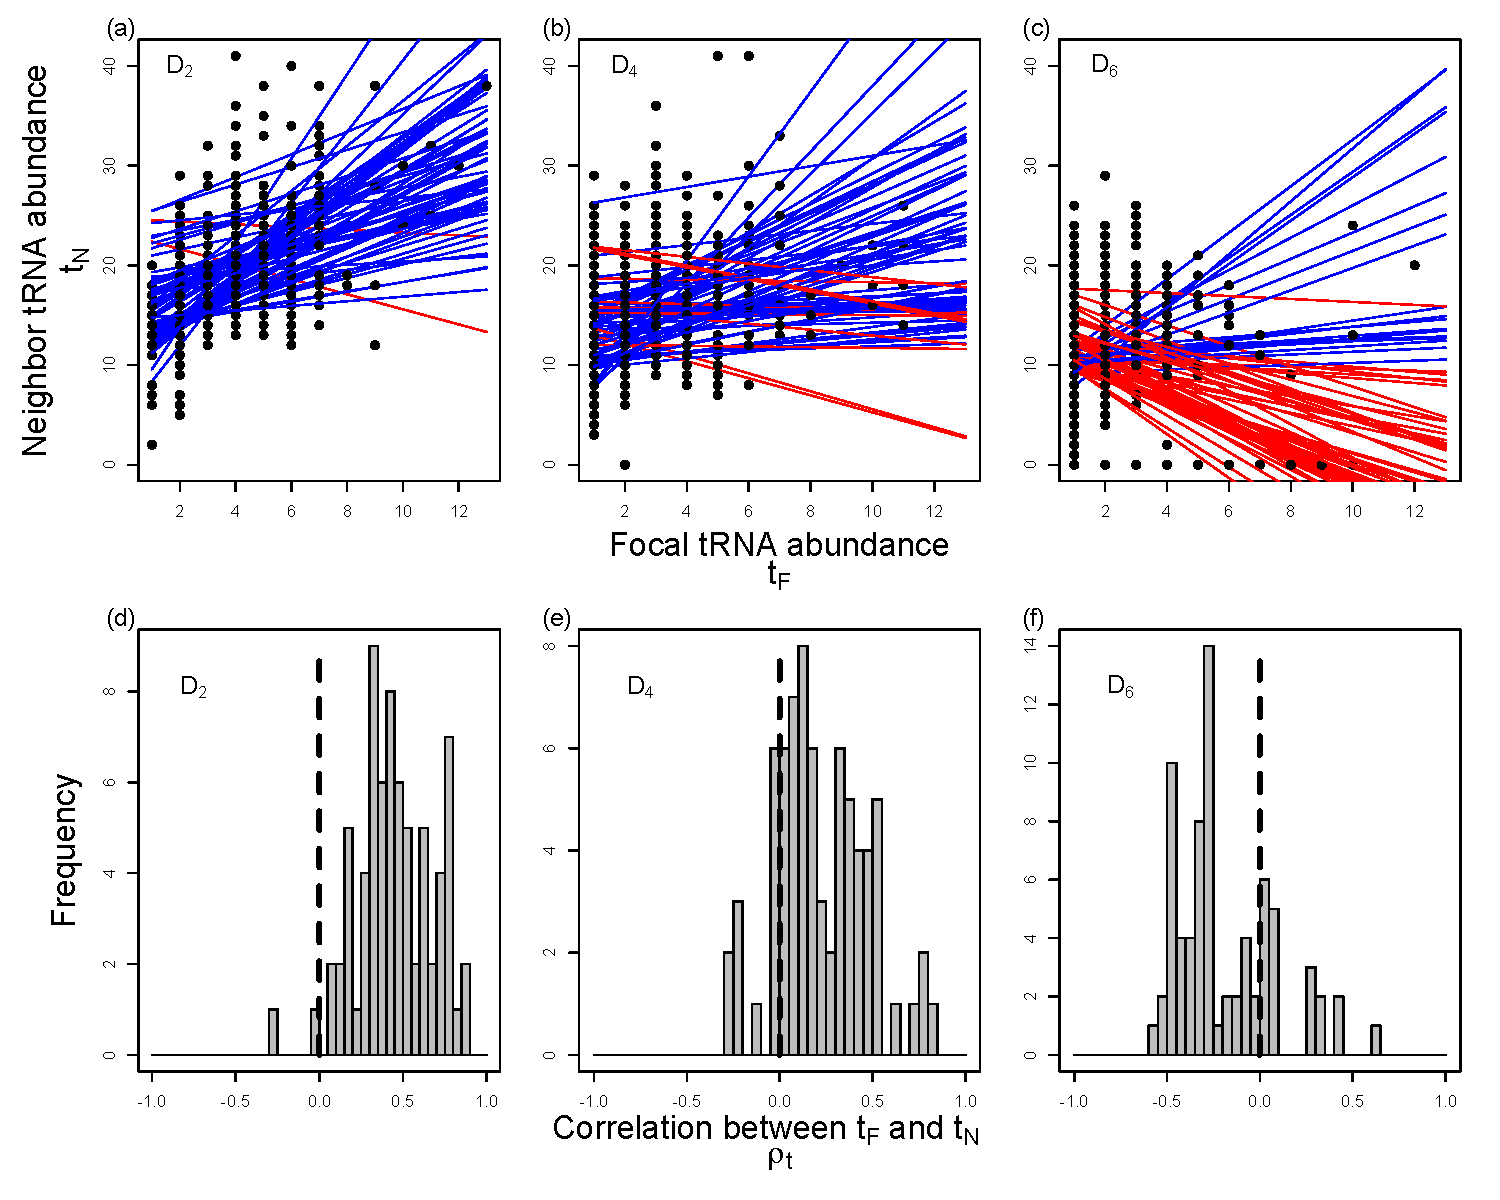
\includegraphics[width=15cm]{../Figure/c2Fig_1.pdf}
	\end{center}
	\caption{{Correlation between a focal tRNA's abundance $t_F$ and the abundance of its neighbors $t_N$, $\rho_t$ across 73 prokaryotic genomes.} }
	Each point in panels (A - C) represents a tRNA species that encodes an amino acid with degeneracy $D_i\, (i=\{2,4,6\})$.
	The solid lines represent the regression lines between $t_F$ and $t_N$ for each genome.
	Genomes with a negative $\rho_t$ are coded in red, while genomes with a positive $\rho_t$ are represented by blue lines.
	Panels (D - F) present the distribution of correlation coefficients $\rho_t$ between $t_F$ and $t_N$  across all the genomes.
	The mean of the distribution of $\rho_t$ values for all the three degenerate classes differ significantly from 0 (Wilcox test, $p<10^{-7}$).
	
	\label{fig:trna.corr}
\end{figure}


We find that the vast majority of genomes (69 out of 73 or $\sim 95\%$) show a positive relationship between the abundance of a focal tRNA species $t_F$ and its one-step non-synonymous neighbors $t_N$, $\rho_t$ (Binomial test, $p<10^{-15}$, Figure \ref{sfig:bs_ec_vp_trna_corr}).

\begin{figure}[H]
	\begin{center}
	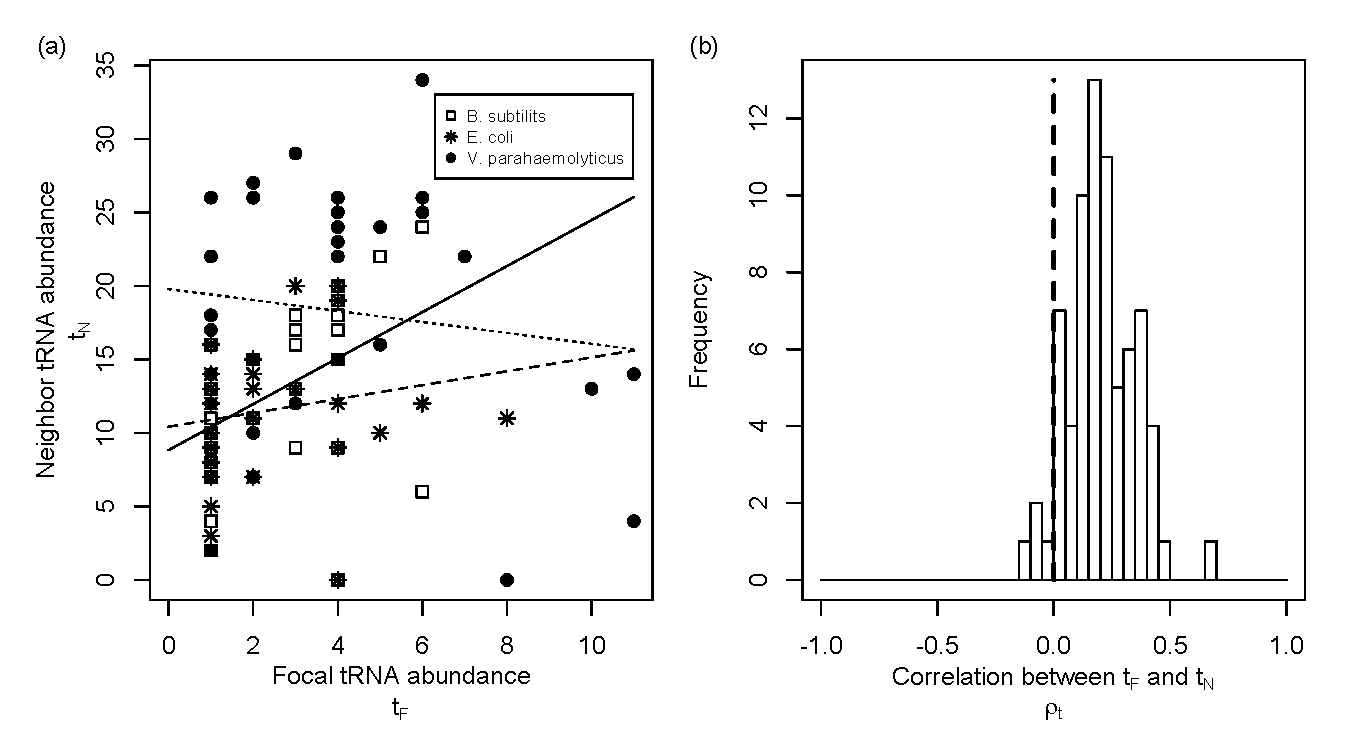
\includegraphics[width=\fullwidth]{../Figure/c2Fig_S1.pdf}
	\end{center}
	\caption{{Correlation between a focal tRNA's abundance $t_F$ and the abundance of its neighbors $t_N$ across prokaryotic genomes.}}
  	Panel (a) represents the correlation between $t_F$ and $t_N$ across all amino acids for \emph{B.~subtilis}, \emph{E. coli} and \emph{V.~parahaemolyticus} .
	Regression line between $t_F$ and $t_N$ for \emph{B.~subtilis}, \emph{E. coli} and \emph{V.~parahaemolyticus} are represented by solid, dashed and dotted lines, respectively.
	Panel (b) shows the distribution of correlation coefficients $\rho_t$ between $t_F$ and $t_N$ across 73 prokaryotic genomes.
	About 69 out of 73 genomes (Binomial test, $p<10^{-15}$) have a positive relationship between $t_F$ and $t_N$.
	
	\label{sfig:bs_ec_vp_trna_corr}
\end{figure}

This indicates that tRNAs with similar abundances are closer to each other in the genetic code than expected under the implicit assumptions of the standard model.
In other words, according to the standard model the tRNA abundances within the genetic code are predicted to be uncorrelated and the distributions of correlation coefficients $\rho_t$  in Figures \ref{fig:trna.corr} (d)-(f) are expected to be centered around $0$.
However, we find that under each of the degenerate classes of amino acids, $D_2$, $D_4$ and $D_6$, the distribution of $\rho_t$ is significantly different from $0$ (Wilcox test, $p<10^{-7} \text{ for all }D_i$).
Interestingly, we also find that the distribution of $\rho_t$ differs considerably between degenerate classes of amino acids.
tRNAs corresponding to amino acids in both $D_2$ and $D_4$ degenerate classes show a significant bias towards a positive correlation between $t_F$ and $t_N$, whereas tRNAs in $D_6$ degenerate class are biased towards a negative correlation.

Since the frequency of amino acid usage within a genome is highly correlated with tRNA gene copy number (e.g.~in \emph{E.~coli} $\rho=0.632$, $p<0.003$), the observed correlations may be the indirect result of amino acid usage bias.
In addition to amino acid usage biases, the stereochemistry of codon-anticodon interactions forbids the existence of certain tRNA types \citep{LimAndCurran01}, potentially contributing to the observed positive correlation among tRNA abundances.
In order to address these inherent constraints on the distribution of tRNAs within the genetic code, we randomly distributed tRNA gene copies taking into account the stereochemical constraints, both with and without biased amino acid usage (see Figures \ref{sfig:trna.corr.nb} and \ref{sfig:trna.corr.aab}).

\begin{figure}[H]
	\begin{center}
	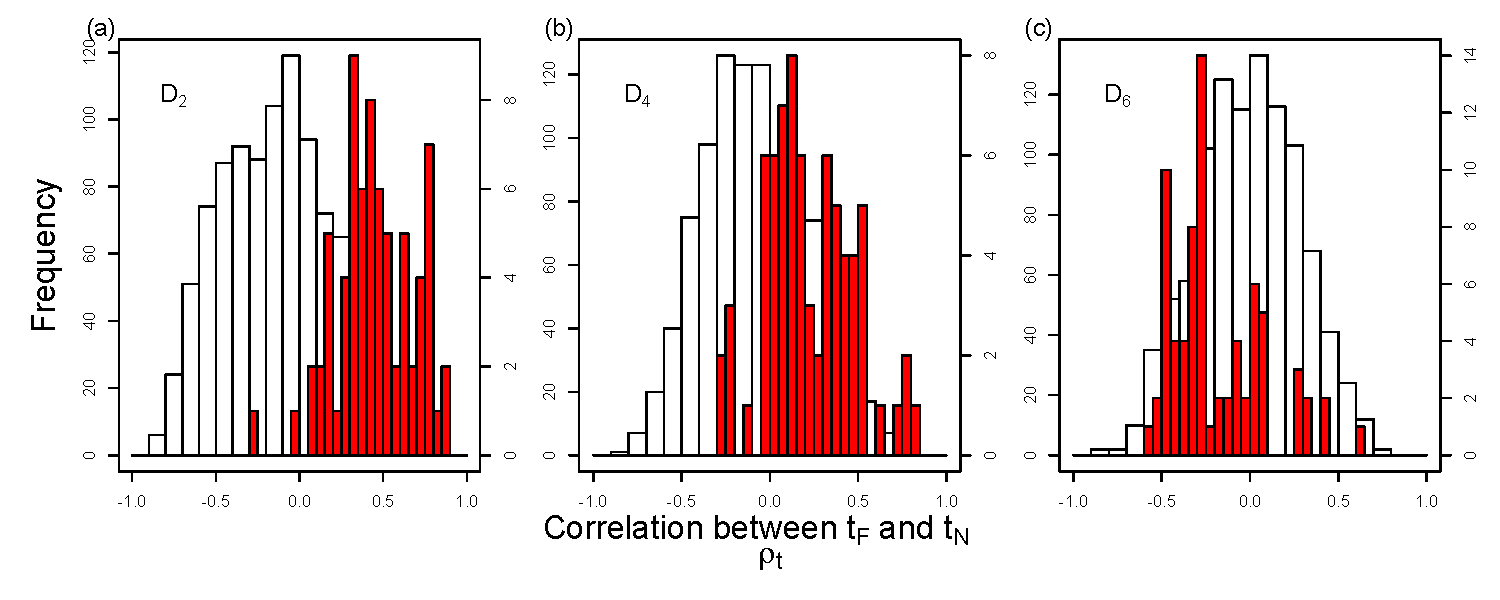
\includegraphics[width=\fullwidth]{../Figure/c2Fig_S3.pdf}
	\end{center}
	\caption{The distribution of correlation coefficients between a focal tRNA's abundance $t_F$ and the abundance of its neighbors $t_N$, $\rho_t$.}
	Open bars represents the null distribution of $\rho_t$ when tRNAs are randomly distributed across the genetic code, taking into account stereochemical constraints on possible tRNA anticodon types.
	Red bars represent the observed distribution of $\rho_t$ across all 73 prokaryotic genomes.
	The observed distribution is significantly different from the null distribution (Kolmogorov-Smirnov test $p<0.001$) across all three degenerate classes.
	
	\label{sfig:trna.corr.nb}
\end{figure}

\clearpage
\pagebreak

\begin{figure}
	\begin{center}
	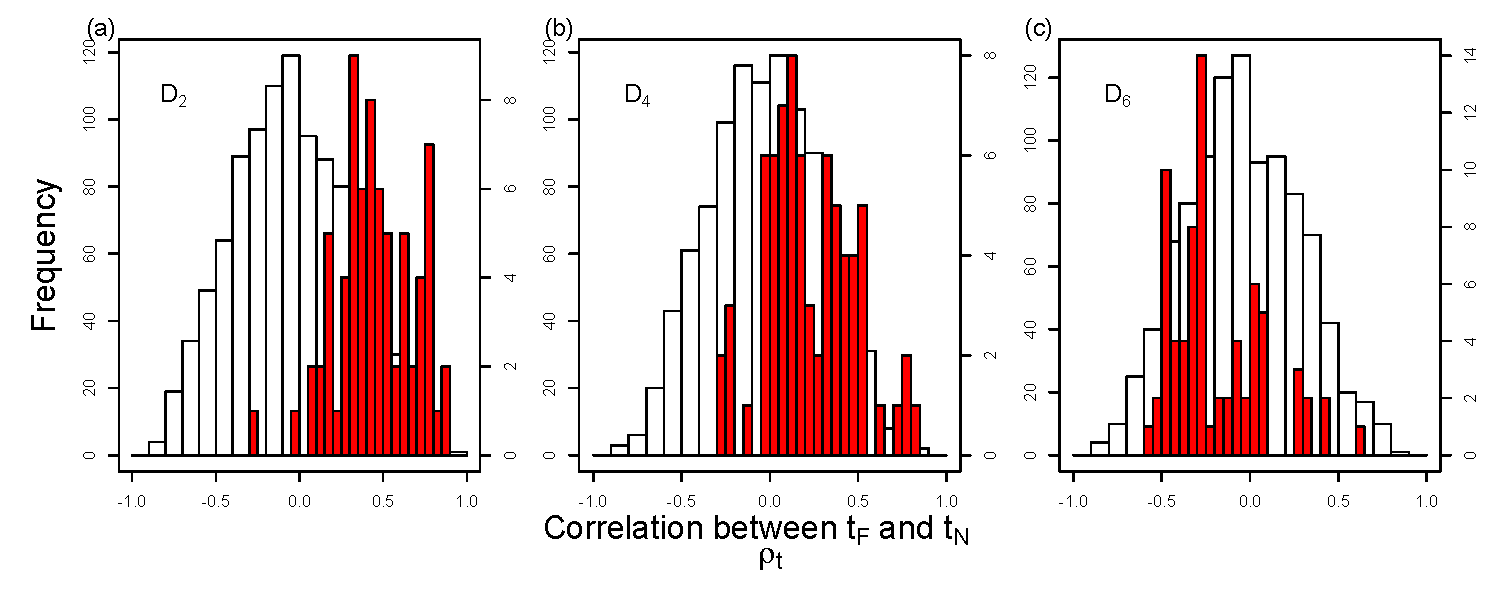
\includegraphics[width=\fullwidth]{../Figure/c2Fig_S4.pdf}
	\end{center}
	\caption{The distribution of correlation coefficients between a focal tRNA's abundance $t_F$ and the abundance of its neighbors $t_N$, $\rho_t$.}
	Open bars represents the null distribution of $\rho_t$ when tRNAs are randomly distributed across the genetic code prop, taking into account stereochemical constraints on possible tRNA anticodon types as well as the observed amino acid frequency distribution in \emph{E. coli} genome.
	Red bars represent the observed distribution of $\rho_t$ across all 73 prokaryotic genomes.
	The observed distribution is significantly different from the null distribution (Kolmogorov-Smirnov test $p<0.001$) across all three degenerate classes.
	
	\label{sfig:trna.corr.aab}
\end{figure}

We find that the observed distribution of $\rho_t$ is significantly different from this more complex null distribution for all of the degenerate classes (Kolmogorov-Smirnov test $p < 0.001$ for all cases).

The distribution of tRNAs within the genetic code have important consequences with respect to translation errors and bias in codon usage.
Codons with higher tRNA abundances than their coding synonyms are often referred to as `optimal' codons \citep{DrummondAndWilke09} assuming they lead to fewer translation errors \citep{Ikemura85, Akashi94, KramerAndFarabaugh07}.
In light of the above results, we now ask the question, ``Given that tRNA abundances are positively correlated in the genetic code, do higher cognate tRNA abundances always lead to fewer translation errors?''

\subsection{Modeling translation errors}
Following \citep{FluittEtAl07}, our model of translation errors takes into account competition between cognate and near-cognate tRNAs for the ribosomal \emph{A}-site during translation.
We also consider the kinetics of tRNA selection within a ribosome \citep{GromadskiAndRodnina04} and the effect of codon-anticodon wobble on these kinetics \citep{CurranAndYarus89}.
During protein translation, when a ribosome waits at a given codon, one of three outcomes is likely to occur: (a) elongation by cognate tRNA, (b) elongation by a near-cognate tRNA leading to a missense error or (c) spontaneous ribosomal drop-off, frameshift or recognition by release factors, any of which will lead to a nonsense error (Figure \ref{fig:translation}).
The relative frequency of each of these outcomes determines the rates of missense and nonsense errors at a particular codon.

\begin{figure}[!ht]
	\begin{center}
	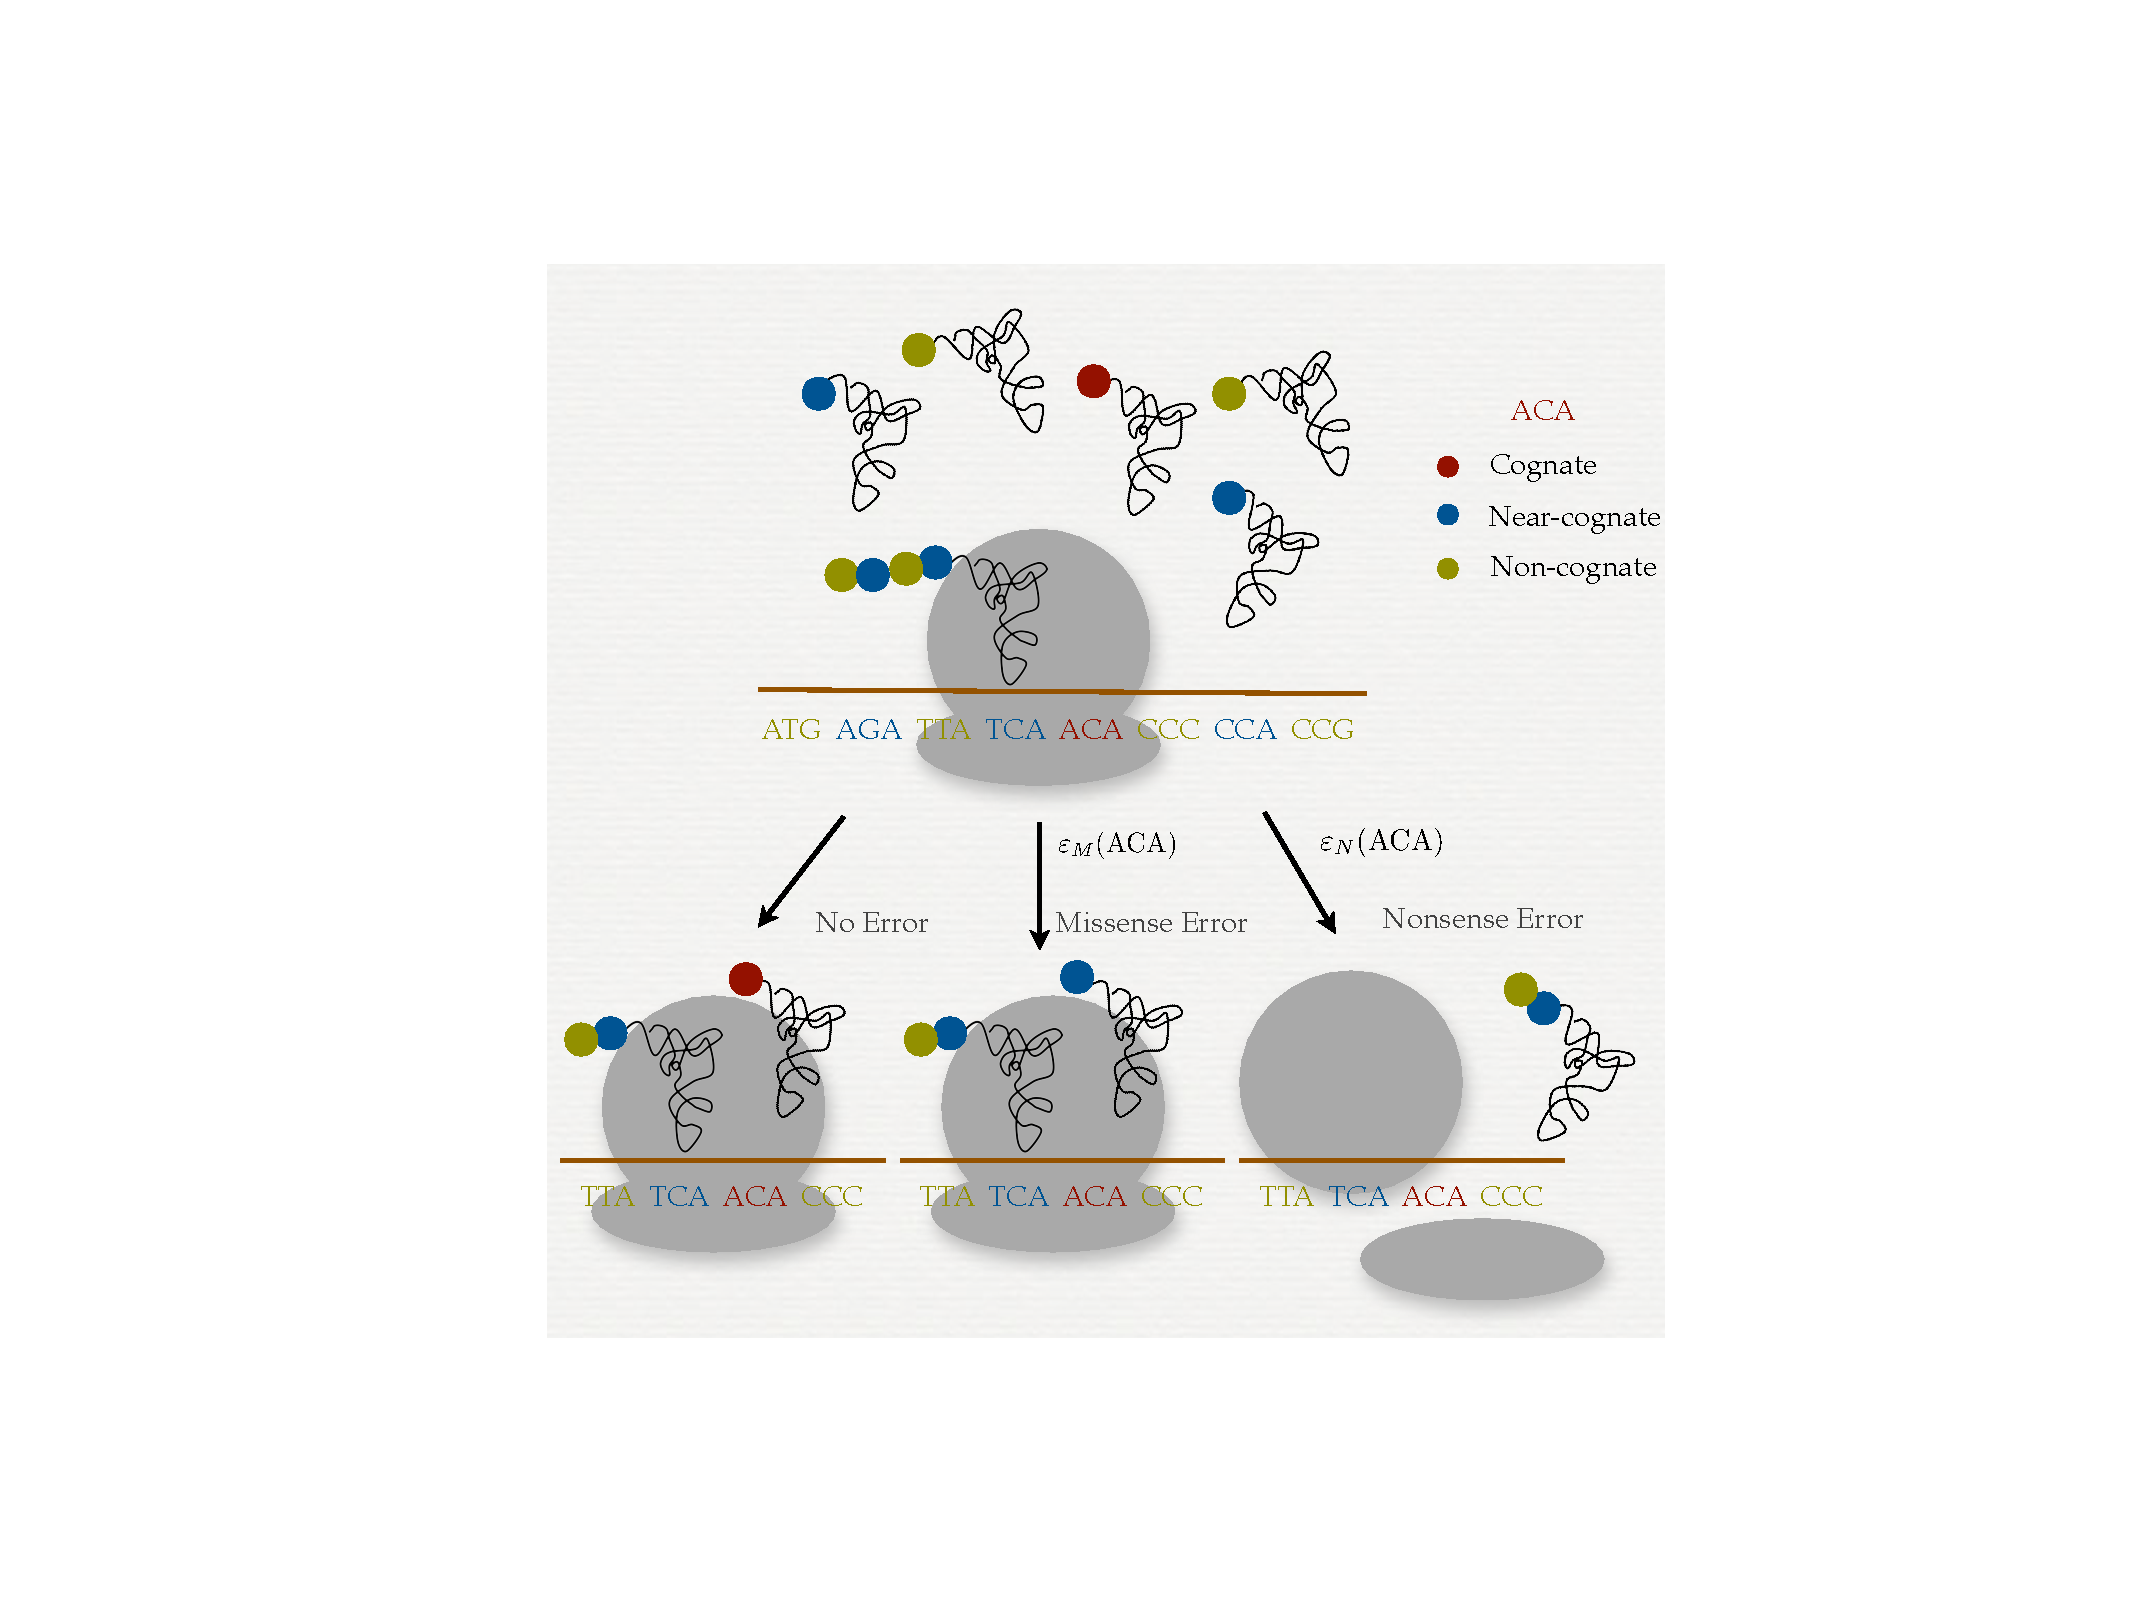
\includegraphics[width=12cm]{../Figure/c2Fig_2.pdf}
	\end{center}
	\caption{{Model of translation errors.}}
	During translation, a ribosome pauses at a codon (ACA in this case) waiting for a cognate tRNA. 
	During this pause, one of the three processes can take place: elongation by cognate tRNAs leading to no translation error, elongation by a near-cognate tRNA leading to a missense error with rate $\varepsilon_M$ or premature termination of translation due to recognition by release factors, spontaneous ribosome drop-off or frameshifting leading to a nonsense error with a rate $\varepsilon_N$.
	
	\label{fig:translation}
\end{figure}


Assuming an exponential waiting process for a tRNA at codon $i$, the codon specific missense and nonsense error rates, $\varepsilon_M$ and $\varepsilon_N$ respectively, can be calculated as follows,
\begin{align}
\varepsilon_M(i)&=\frac{R_\text{n}(i)}{R_\text{c}(i)+R_\text{n}(i)+R_\text{d}}\\
\varepsilon_N(i)&=\frac{R_\text{d}}{R_\text{c}(i)+R_\text{n}(i)+R_\text{d}}
\end{align}
where $R_c(i)$ is the codon specific cognate elongation rate, $R_n(i)$ is the codon specific near-cognate elongation rate, and $R_d$ represents the background nonsense error rate (see \emph{Methods} for details).

Using Equations (1) and (2), we calculated codon-specific missense and nonsense error rates for each bacterial genome.
In order to understand the effect of codon degeneracy on the relationship between error rates and codon elongation rates, we categorized amino acids based on the number of their synonymous codons $D_i$ as before.
Given our model was parametrized from data on \emph{E.\ coli}, we also checked for the sensitivity of our analysis to changes in these parameters when extending it to other prokaryotes (Section \ref{sec:parm.sens}).

\subsection{Error Rates vs. Elongation Rates}
Using \emph{E.\ coli} strain K12/DH10B (K12) as an example, our estimates of codon-specific missense error rates $\varepsilon_M$ ranged from $0-9.38\times 10^{-3}$ with a median of $2.50\times10^{-3}$.
Six of the 61 sense codons have a predicted missense error rate of $0$ as these codons have no near-cognate tRNA species (Table \ref{stable:ecoli.tRNA}).

\begin{table}[H]
\caption{List of codon-specific tRNAs, elongation rates and error rates in $E.~coli$ }
\label{stable:ecoli.tRNA}
\centering
                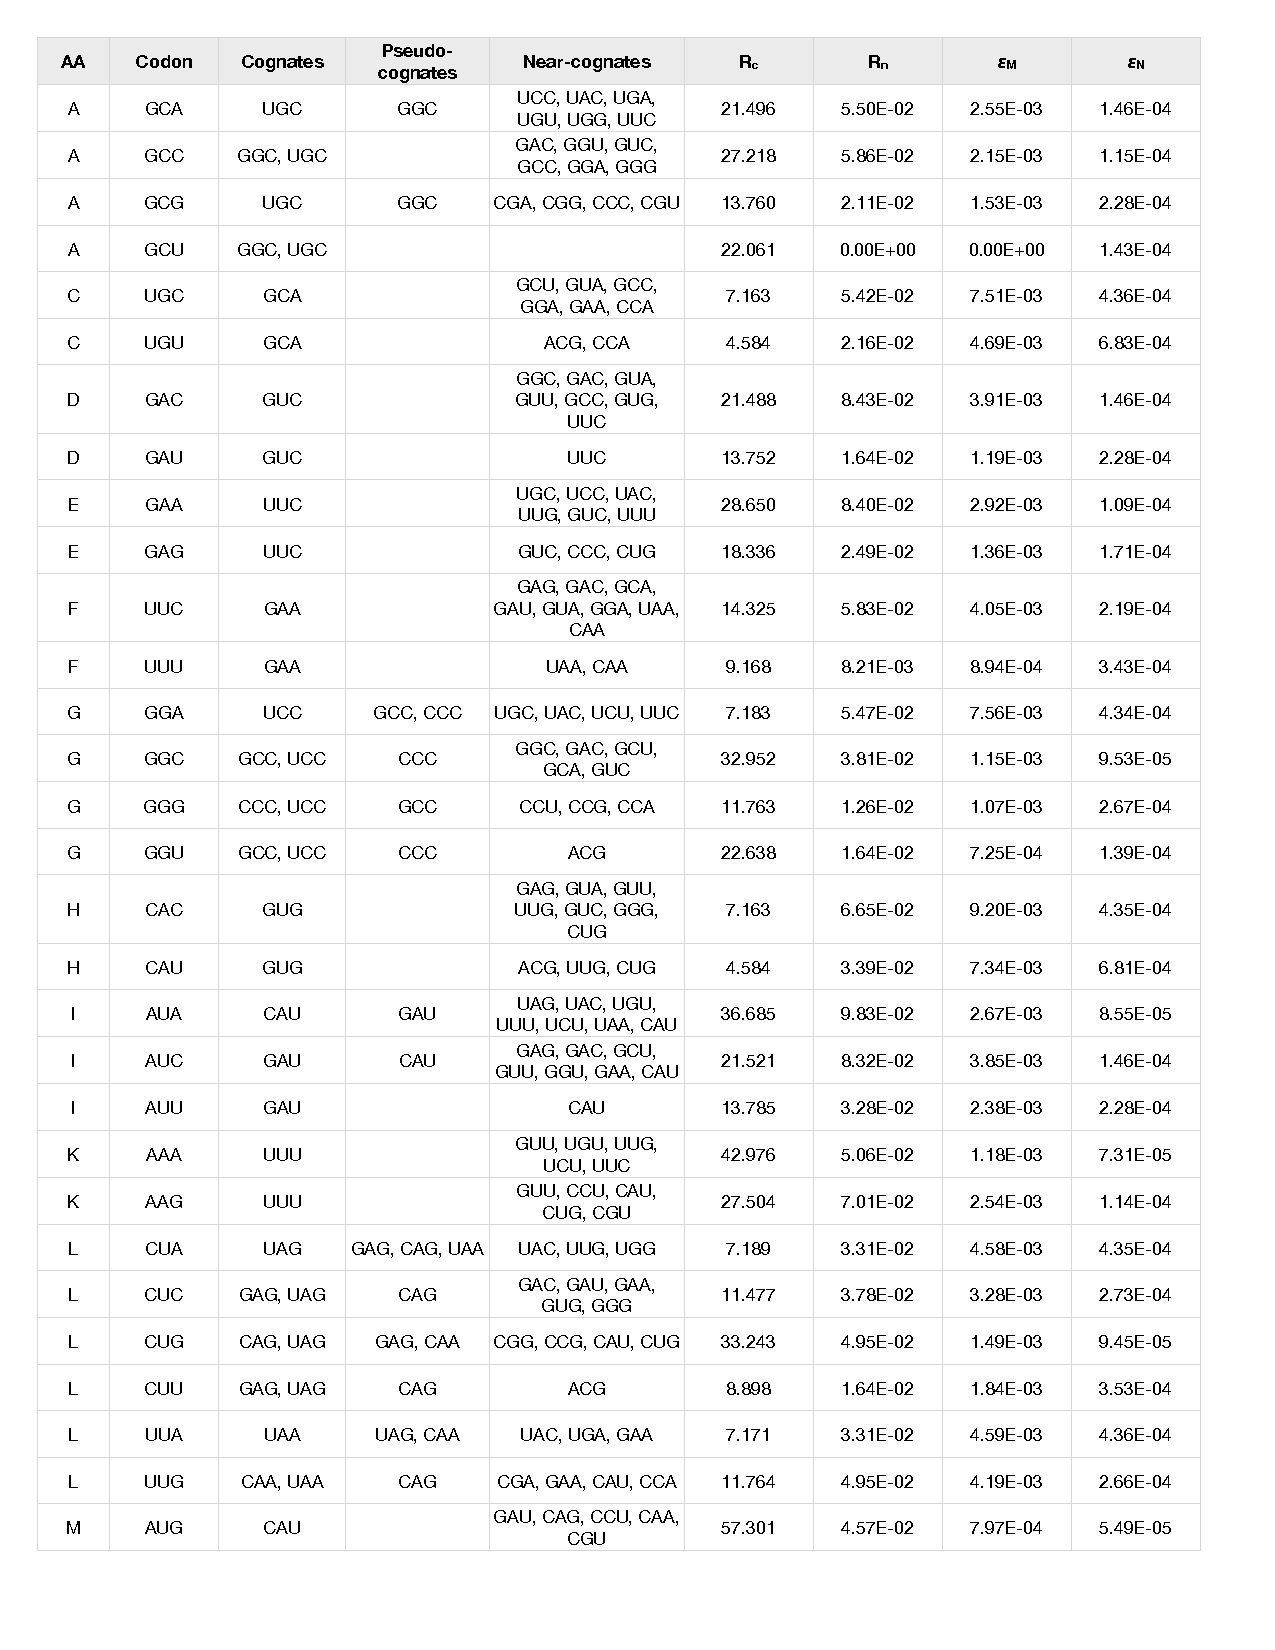
\includegraphics[width=\fullwidth]{../Figure/c2Tab_S2_1.pdf}
%\endhead
\end{table}
%\thispagestyle{empty}
\addtocounter{table}{-1}
\begin{table}
%\clearpage
%\pagebreak
\caption{(continued)}
       \centering
                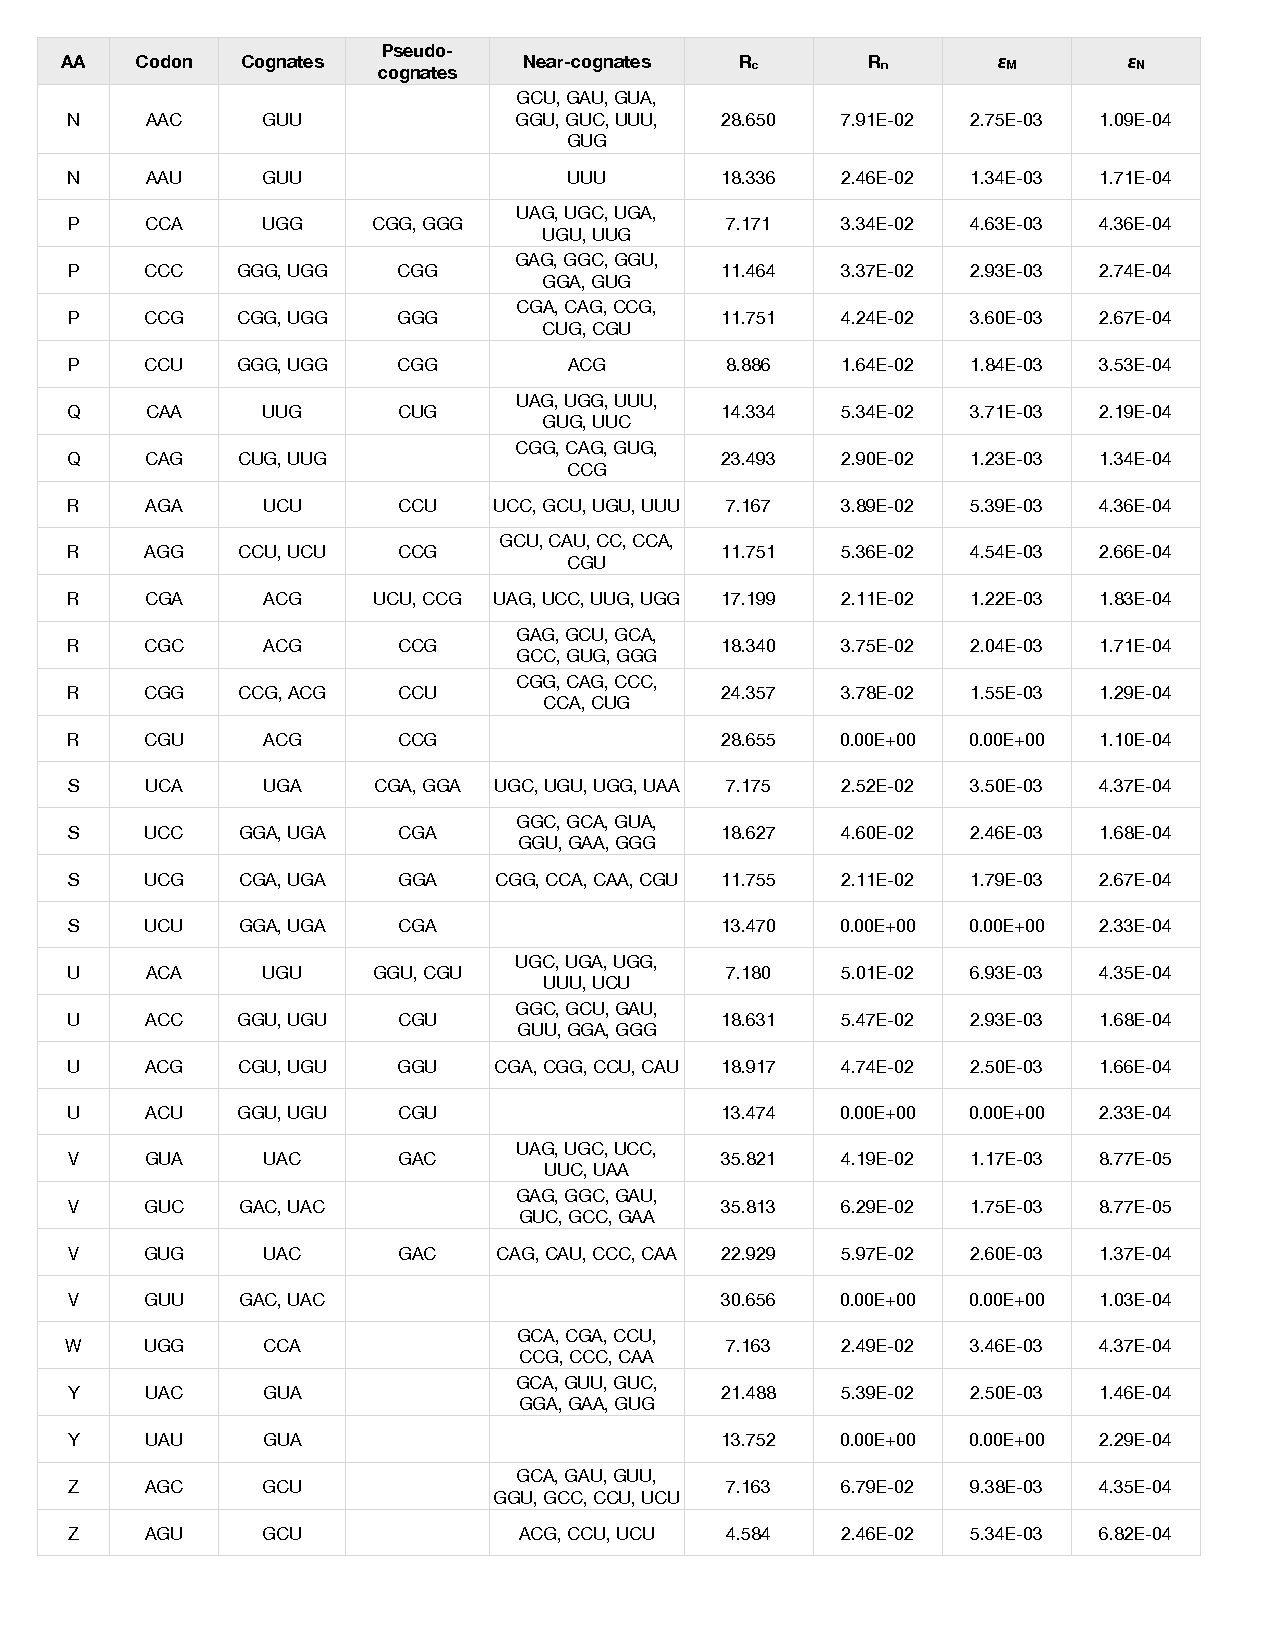
\includegraphics[width=\fullwidth]{../Figure/c2Tab_S2_2.pdf}
\end{table}


These rates are higher than recent empirical estimates of missense error rates in \emph{E.\ coli}, which vary from $2.0\times10^{-4}-3.6\times10^{-3}$ with a median value of $3.4\times10^{-4}$ \citep{KramerAndFarabaugh07}.
This is likely due to the fact that the missense error estimates in \citep{KramerAndFarabaugh07} were for specific amino acid misincorporations, whereas, the values predicted here indicate the rate of all possible missense errors at a given codon.
Our predicted rates of codon-specific nonsense errors $\varepsilon_N$ in \emph{E.\ coli} ranged from $5.49\times10^{-5}-6.83\times10^{-4}$ with a median of $2.19\times10^{-4}$ (Table \ref{stable:ecoli.tRNA}).

We find that on average both missense $\varepsilon_M$ and nonsense error rates $\varepsilon_N$ decrease with an increase in cognate elongation rates $R_c$ (Figure \ref{fig:miss.nons.rc}).

\begin{figure}[H]
	\begin{center}
	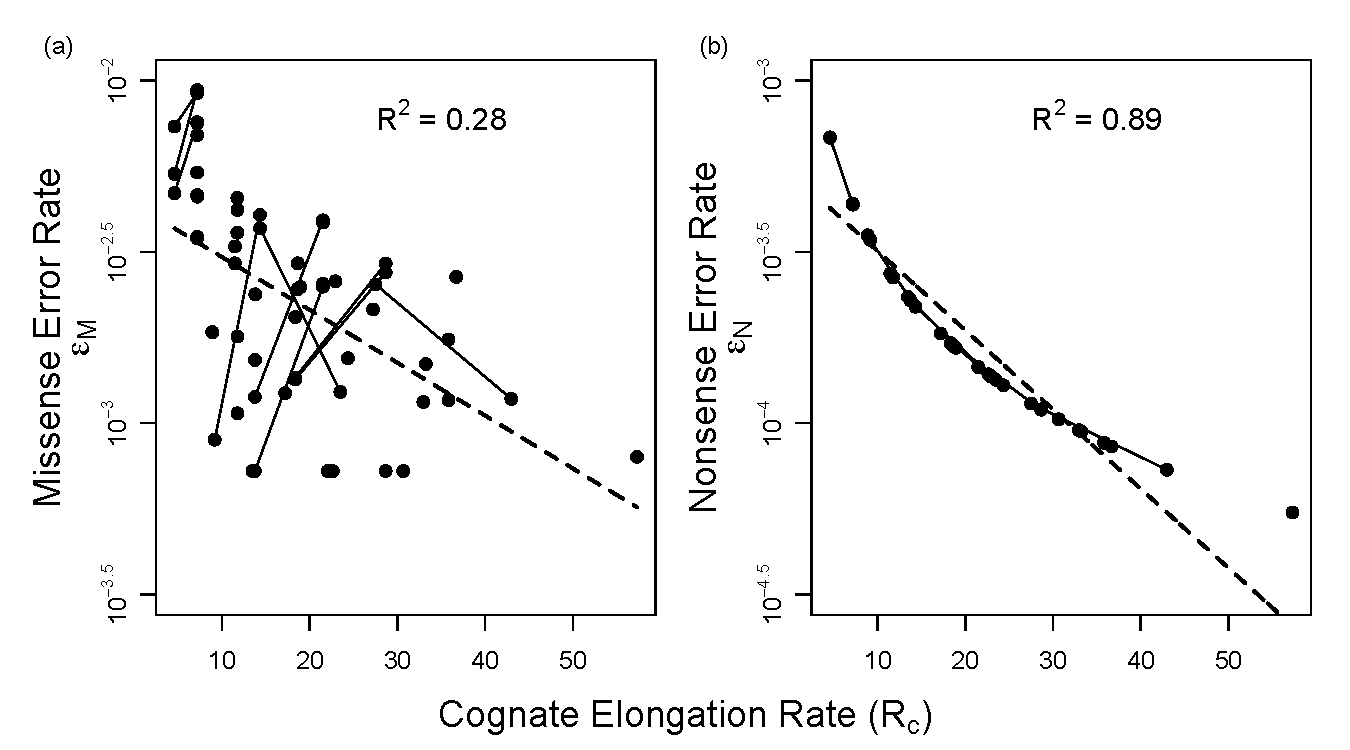
\includegraphics[width=15cm]{../Figure/c2Fig_3.pdf}
	\end{center}
	\caption{{Correlation of translation error rates $\varepsilon$ with cognate elongation rate $R_c$ in \emph{E. coli}.}}
	We find that rates of both (A) missense $\varepsilon_M$ and (B) nonsense errors $\varepsilon_N$ are negatively correlated with the rate of elongation by cognate tRNAs at that codon.
	The dashed line indicates the regression line between $R_c$ and $\varepsilon$.
	This is consistent with expectations under the standard model.
	However, in the case of twofold degenerate amino acids ($D_2$), whose two codons are joined together by solid lines, we see that $\varepsilon_M$ increases with $R_c$ for 8 out of 10 amino acids.
	In the case of $\varepsilon_N$ every amino acid showed a decrease in $\varepsilon_N$ with $R_c$.
	
	\label{fig:miss.nons.rc}
\end{figure}

These results seem, on first glance, largely consistent with the standard model for inferring translation errors from tRNA abundances, which assumes that $\varepsilon$ decreases with $R_c$.
However, because $R_n$ varies between synonymous codons, for about half of the amino acids (10 out of 21) $\varepsilon_M$ is actually greater for the codon with the highest $R_c$ value.
This holds even when empirical estimates of tRNA abundances in \emph{E. coli} \citep{DongEtAl96} are used instead of tRNA gene copy numbers (see Figure \ref{sfig:corr.empirical}).


\begin{figure}[H]
	\begin{center}
	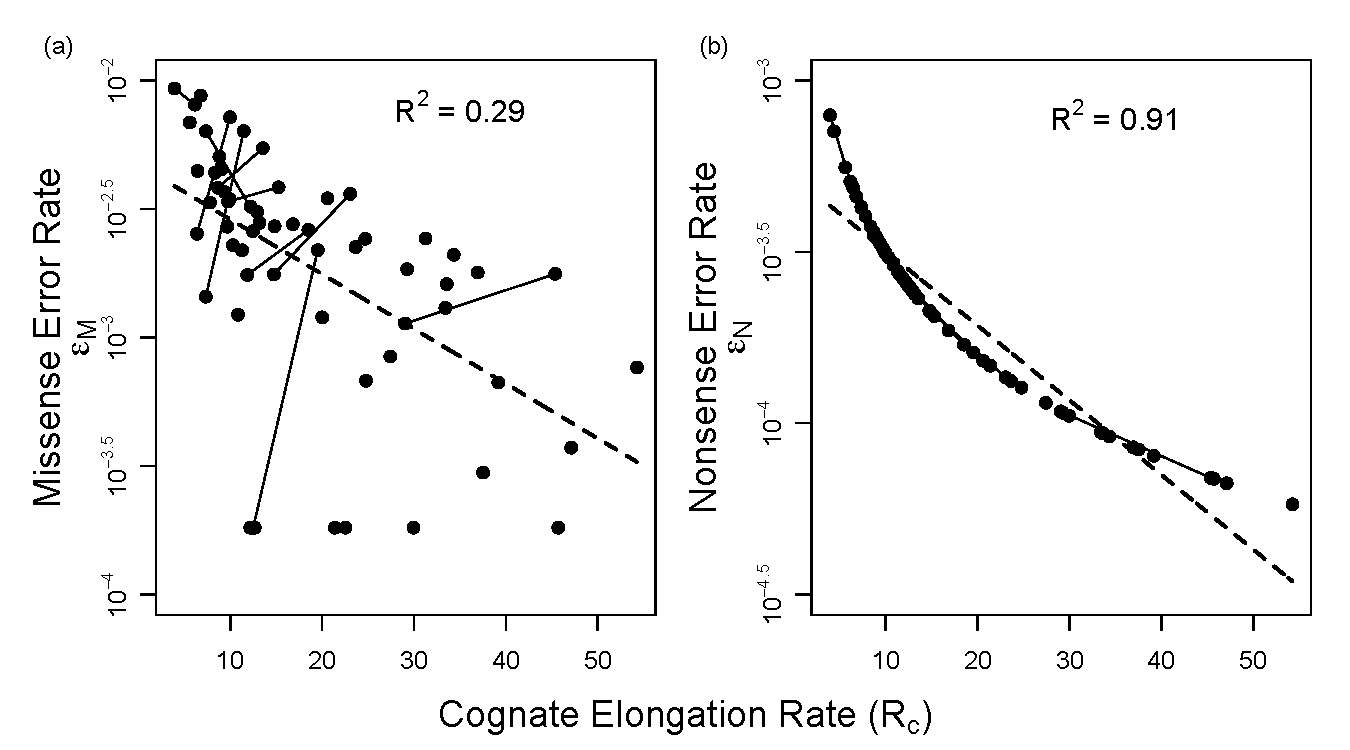
\includegraphics[width=\fullwidth]{../Figure/c2Fig_S5.pdf}
	\end{center}
	\caption{Correlation of translation error rates $\varepsilon$ with cognate elongation rate $R_c$ using empirical estimate of tRNA abundances.}
	We find that rates of both (a.) missense $\varepsilon_M$ and (b.) nonsense errors $\varepsilon_N$ are negatively correlated with the rate of elongation by cognate tRNAs at that codon.
	The dashed line indicates the regression line between $R_c$ and $\varepsilon$.
	These results are consistent with the results obtained using tRNA gene copy numbers as proxies for tRNA abundances.
	
	\label{sfig:corr.empirical}
\end{figure}

This result is \emph{inconsistent} with expectations under the standard model that implicitly assumes a codon-independent rate of elongation by near-cognate tRNAs, $R_{n}$.
If the abundance of a focal tRNA $t_F$ and its neighbors $t_N$ are uncorrelated, then the only factor that affects $\varepsilon_M$ is $R_c$.
However, as shown earlier, $t_F$ and $t_N$ are positively correlated (Figure \ref{fig:trna.corr}).
Thus, the estimates of $\varepsilon_M$ of synonymous codons of an amino acid depend not only on their individual $R_c$ but also on the slope of the relationship between $R_c$ and $R_n$.
If the rate of increase of $R_n$ with $R_c$ is higher than the relative increase in $R_c$, then codons with higher cognate elongation rates $R_c$ are expected to have \emph{higher} missense error rates $\varepsilon_M$ (Figure \ref{sfig:contourplot}).

\begin{figure}[H]
	\begin{center}
	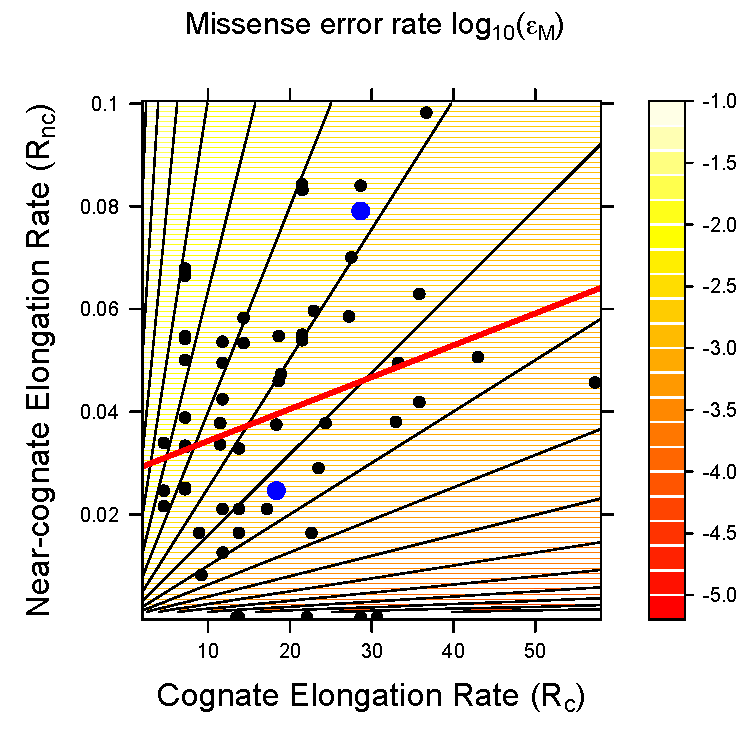
\includegraphics[width=\fullwidth]{../Figure/c2Fig_S2.pdf}
	\end{center}
	\caption{Contour plot of missense error rates $\text{log}_{10}(\varepsilon_M)$ with cognate $R_c$ and near-cognate $R_n$ elongation rates.}
  	The black dots represent $\text{log}_{10}(\varepsilon_M)$ of codons in $E.~coli$.
  	Blue dots are the two codons of amino acid asparagine (N). 	
	In the case of asparagine, the codon with a higher $R_c$ has a higher $\varepsilon_M$ as it also has  a much higher $R_{n}$.
	The regression line between observed $R_{c}$ and $R_{n}$ in $E.~coli$ is represented as a solid red line.
	The positive correlation between $R_c$ and $R_{n}$, explains why codons with higher $R_c$ sometimes have a higher missense error rate.
	
	\label{sfig:contourplot}
\end{figure}

Interestingly, 8 out of the 10 $D_2$ amino acids in \emph{E.\ coli} K12 showed a positive relationship between $R_c$ and $\varepsilon_M$.
Specifically, we would expect $\varepsilon_M$ to increase with $R_c$ whenever the condition $\frac{dR_n}{dR_c}>\frac{R_n}{R_c}$ is satisfied. 
Thus, among the synonymous codons of an amino acid  in \emph{E.\ coli}, the codon with the lowest $\varepsilon_M$ is often not the codon with the highest $R_c$.
This points to a fundamental change in our understanding of the relationship between tRNA abundances and missense errors and which codons minimize their occurrence.

Interestingly, these results are also consistent with the limited empirical estimates of codon-specific missense error rates.
For instance, \citep{PrecupAndParker87} used \emph{E.~coli} to estimate rates at which the asparagine codons AAC and AAU were mistranslated by  $\text{tRNA}^\text{Lys}_\text{UUU}$.
As expected, the authors found that the AAC codon, with a higher $R_c$ had a lower rate of mistranslation by $\text{tRNA}^\text{Lys}_\text{UUU}$ than AAU, with a lower $R_c$.
Our model makes the same prediction when considering this specific subset of missense errors.
However, when considering the overall missense error rates at AAC and AAU codons due to $\text{tRNA}^\text{Lys}$, $\text{tRNA}^\text{Ser}$, $\text{tRNA}^\text{Thr}$, $\text{tRNA}^\text{Asp}$, $\text{tRNA}^\text{His}$, $\text{tRNA}^\text{Tyr}$ and $\text{tRNA}^\text{Ile}$(all one-step neighbors), we come to a very different prediction.
Specifically we find that even though AAC has a higher $R_c$ than AAU, it also has a much higher $R_n$ rate. 
As a result, the \emph{overall} missense error rate for AAC is actually predicted to be higher than AAU. 
This result illustrates how focusing on only a subset of possible missense errors at a codon, as all previous experiments have done, provides an incomplete and potentially misleading picture.

In contrast to missense error rates, our model predicts $\varepsilon_N$ will consistently decline with an increase in $R_c$, suggesting that nonsense errors may be playing a larger role in driving CUB than commonly accepted \citep{AravaEtAl05}.

\subsection{Intra- and Inter-specific Variation in the Relationship between Elongation and Error Rates}
In order to evaluate the relationship between cognate elongation rate, $R_c$, and error rates, we looked across 73 bacterial genomes for inter-specific variation and 11 strains of \emph{E.\ coli} for intra-specific variation.
As before, we categorized amino acids 
based on the degeneracy of their synonymous codons for each genome.
%Under the standard model where the abundances of tRNAs are assumed to be uncorrelated, we expect to observe a negative relationship between $R_c$ and translation errors.
We calculated the fraction of amino acids within each category that showed a \emph{negative} relationship between $R_{c}$ and error rates, $\varepsilon_M$ and $\varepsilon_N$ (Figure \ref{fig:8panel}) as expected under the standard model where the abundances of tRNAs are assumed to be uncorrelated.

\begin{figure}[!ht]
	\begin{center}
	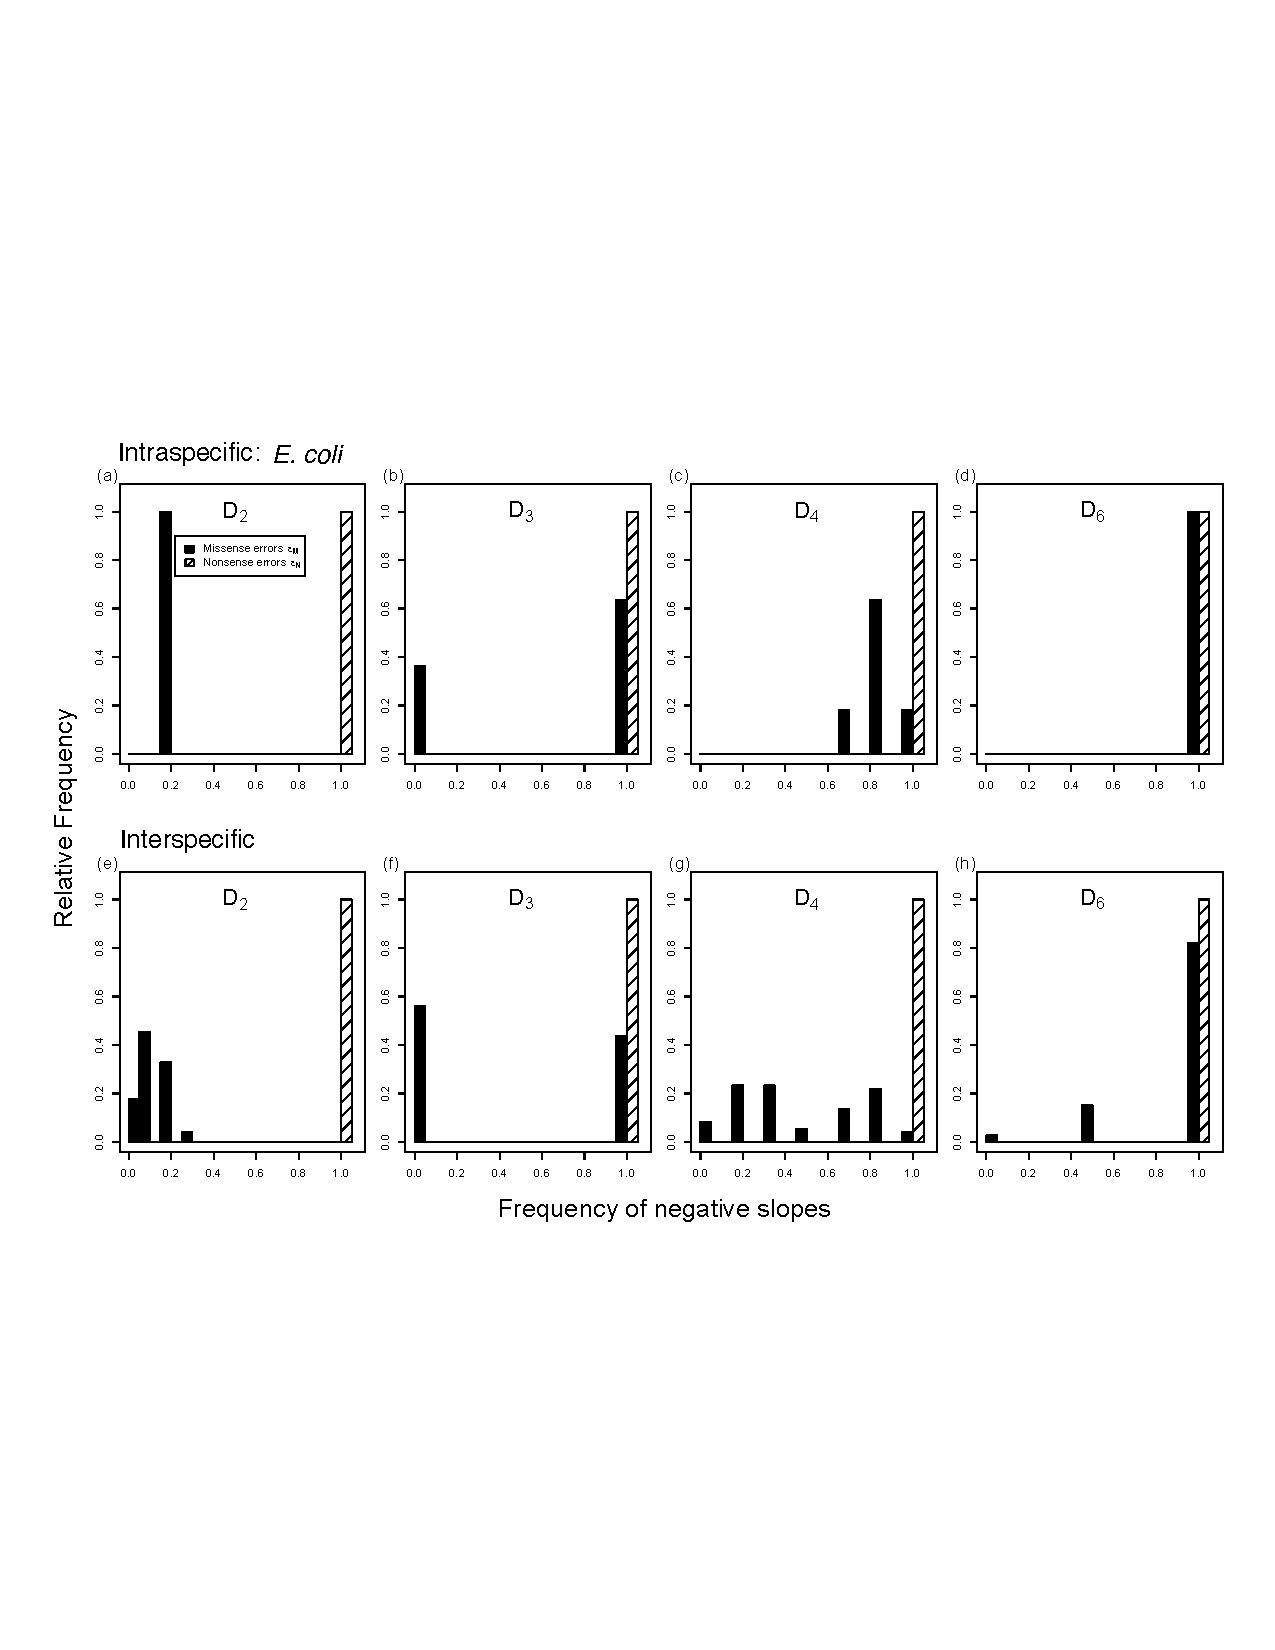
\includegraphics[width=15cm]{../Figure/c2Fig_4.pdf}
	\end{center}
	\caption{{Frequencies of negative relationships between cognate elongation rate $R_c$ and translation errors $\varepsilon$.}}
	Panels (A - D) represent the distribution of \emph{E. coli} strains that show amino acid specific negative relationship between $R_c$ and $\varepsilon$, while panels (E - H) represent the distribution of 73 genomes for the same.
	Amino acids in every degenerate class ($D_i$) show a negative relationship between cognate elongation rate $R_c$ and nonsense error rates ($\varepsilon_N$) both intra-specifically as well as inter-specifically.
	A majority of amino acids in the 2-fold degenerate class ($D_2$) show an increase in missense error rate $\varepsilon_M$ with $R_c$ across genomes.
	As the degeneracy of amino acids increases, we see an increase in the frequency of the expected negative relationship between $\varepsilon_M$ and $R_c$ across \emph{E.\ coli} strains as well as other bacterial species.
	
	\label{fig:8panel}
\end{figure}

For both intra- and inter-specific datasets we find that synonymous codons with a higher $R_c$ have a lower nonsense error rate $\varepsilon_N$ for all amino acids, irrespective of the degenerate class $D_i$ they belong to.
However, in the case of missense errors, the relationship between $R_c$ and $\varepsilon_M$ depends on the amino acid degeneracy $D_i$ as previously observed in \emph{E.\ coli} K12 (Figure \ref{fig:miss.nons.rc}).
Amino acids with two synonymous codons ($D_2$) show a strong bias towards a \emph{positive} relationship between $R_c$ and $\varepsilon_M$, both intra- and inter-specifically (Binomial test, $p=1.5\times10^{-10}$ and $p<2.2\times10^{-16}$, respectively).
In the case of isoleucine, the only amino acid in $D_3$, there exists no bias towards a positive or a negative relationship between cognate elongation and missense error rates (Binomial test, intra-specific $p=0.548$ and interspecific $p=0.349$).
Interestingly 4-fold degenerate amino acids show a bimodal distribution of the fraction of genomes with a negative relationship, and the two 6-fold degenerate amino acids (arginine and leucine) show a strong bias towards negative correlation between $R_c$ and $\varepsilon_M$  (Binomial test, intra-specific $p=4.7\times10^{-7}$ and interspecific $p<2.2\times10^{-16}$).
The differences in the relationship between $\varepsilon_M$ and $R_c$ across degenerate classes are similar to the differences in the correlation between $t_F$ and $t_N$ across these classes (Figure \ref{fig:trna.corr}).

Although the patterns we observe are complex and vary with amino acid degenerate classes, the assumption underlying the standard model that higher cognate tRNA abundance codons will have the lowest translation error rates is predicted to be clearly violated in the case of missense errors -- a finding consistent both across bacterial genomes and across various \emph{E.\ coli} strains.
We also find that the positive relationship between missense error rates $\varepsilon_M$ and $R_c$ observed within certain amino acids is insensitive to moderate changes in parameter estimates of background nonsense error rates, and wobble parameters (Section \ref{sec:parm.sens}).

\section{Discussion}
For over 30 years, the standard model of translation errors has implicitly assumed that for any given amino acid, the translation error rates are lowest for the codons with the highest tRNA abundances \citep{Ikemura81, VarenneEtAl84, KramerAndFarabaugh07}.
With respect to missense errors $\varepsilon_M$, this prediction was based on the implicit and unstated assumption that the distribution of tRNA abundances across the genetic code are uncorrelated.
Here we show a consistent positive correlation between the abundance of a tRNA and its one-step mutational neighbors across a wide array of prokaryotes.
In order to understand the effects of this relationship on translation errors, we developed a simple model for estimating codon-specific error rates based on the distribution of tRNA gene copy number of a species.
Our model takes into account tRNA competition, wobble effects, and intra-ribosomal kinetics of elongation to predict rates of missense and nonsense errors.
To our knowledge, ours is the first model to integrate all these factors for estimating translation errors.
Using our model, we find that on \emph{average}, both missense and nonsense error rates of a codon decrease with an increase in its cognate tRNA elongation rate.
This average behavior is consistent with expectations under the standard model of how codon specific error rates scale with cognate tRNA abundance \citep{Akashi94, StoletzkiAndEyreWalker07, KramerAndFarabaugh07, DrummondAndWilke08}.
However, the expected relationship between error rates and cognate tRNA abundances does not hold at finer scales of individual amino acids, the relevant scale for the evolution of CUB.

For about half of the amino acids (10 out of 21) in \emph{E.\ coli} K12, synonymous codons that have higher cognate elongation rates $R_c$ also have higher missense error rates $\varepsilon_M$.
This counterintuitive behavior is due to the fact that tRNA abundances within the genetic code are positively correlated, which leads to an increase in $\varepsilon_M$ with $R_c$, an important pattern that has been overlooked by previous researchers.
We find a positive correlation between the abundance of a focal tRNA $t_F$ and that of its neighbors $t_N$ in 69 out of 73 genomes examined here.
In addition, the 4 genomes that show a negative $\rho_t$ (\emph{E. coli} O157H7, \emph{E. coli} O157H7-EDL933,  \emph{Photobacterium profundum} SS9, \emph{Vibrio parahaemolyticus}) also show evidence of a high degree of horizontal gene transfer.
Interestingly we also find that the differences in the relationship between $t_F$ and $t_N$ across amino acid degenerate classes is mirrored in the correlation between $\varepsilon_M$ and $R_c$.
In contrast to $\varepsilon_M$, the nonsense error rates $\varepsilon_N$ of synonymous codons decrease with an increase in $R_c$ for every amino acid across every genome we analyzed. 
This is due to the fact that increasing either $R_c$ or $R_n$ leads to a decrease in ribosomal wait time at that codon which, in turn, leads to a lower $\varepsilon_N$.
Thus with respect to $\varepsilon_N$, a positive correlation between tRNA abundances actually accentuates the advantage of using codons with higher tRNA abundances.
These results lend further support to the hypothesis that nonsense errors play an important but under-appreciated role in the evolution of CUB \citep{Gilchrist07,GilchristEtAl09}.

The role of tRNA competition has been recognized as an important factor in affecting translation error rates \citep{VarenneEtAl84, FluittEtAl07, KramerAndFarabaugh07}.
However, previous studies on the relationship between error rates and tRNA abundances have focused primarily on the effects of modifying cognate tRNA abundances and ignored the effects of near-cognate tRNA abundances.
Consistent with our model behavior, \citep{KramerAndFarabaugh07} showed that when $\text{tRNA}^\text{Arg}_\text{UCU}$ was over-expressed, it led to a decrease in the missense error rate $\varepsilon_M$ at codons for which the tRNA was a cognate: AGA and AGG.
However, if a higher expression level of $\text{tRNA}^\text{Arg}_\text{UCU}$ reduces the frequency of $\varepsilon_M$ at codons AGA and AGG, why is it not fixed in the population?
We argue that increasing the abundance of a given tRNA may not always be adaptive.
For instance, over-expressing $\text{tRNA}^\text{Arg}_\text{UCU}$ will also lead to an increase in $\varepsilon_M$ at nearby non-synonymous codons - AAA, ACA, AUA, etc., a testable prediction not considered by \citep{KramerAndFarabaugh07}.
The trade-offs between reducing $\varepsilon_M$ at one codon at the expense of increasing $\varepsilon_M$ at nearby codons has not been explored.
However, these trade-offs likely play an important role in shaping the evolution of tRNA gene copy number and force us to reconsider the evolutionary causes of CUB.

Currently, many researchers believe that selection for translational accuracy, i.e., against missense errors, is a primary force driving the evolution of CUB (see \citep{Akashi94, AravaEtAl05, DrummondEtAl05, StoletzkiAndEyreWalker07}).
This belief largely rests on the interpretation of two facts.
Firstly, preferred codons are generally those with the highest corresponding tRNA abundances  and secondly, sites that are highly conserved and thought to have large effects on protein structure and function, use preferred codons more often than their coding synonyms \citep{Akashi94}.
Selection for translational accuracy is usually tested using Akashi's test by identifying evolutionarily conserved sites in protein sequences and checking whether they are coded by preferred codons \citep{Akashi94, DrummondEtAl06, StoletzkiAndEyreWalker07, DrummondAndWilke09}.
In light of the above results, we need to revisit the underlying assumptions of Akashi's test \citep{Akashi94}.
Although, our analysis predicts that a considerable number of amino acids have a positive relationship between missense error rates, $\varepsilon_M$ and cognate elongation rates $R_c$, many amino acids in $E.~coli$ are still predicted to conform to the standard model of lower $\varepsilon_M$ with higher $R_c$.
Indeed, in the case of \emph{Drosophila} species used in the original Akashi's paper \citep{Akashi94}, only 4 out of 21 amino acids are predicted to have a positive relationship between $\varepsilon_M$ and $R_c$.
Thus, we argue that the relationship between $\varepsilon_M$ and $R_c$ are highly species and amino acid specific and that selection for translation accuracy cannot explain all of the observed CUB at conserved sites.
In addition to selection for translational accuracy, selection against nonsense errors \citep{GilchristAndWagner06, Gilchrist07, GilchristEtAl09}, mRNA stability \citep{Bulmer91} and protein misfolding due to ribosome stalling \citep{KimchiSarfatyEtAl07, TsaiEtAl08} have been shown to affect CUB.
In fact, recent evidence suggests that the speed of translating a codon also affects protein folding \citep{KimchiSarfatyEtAl07, TsaiEtAl08, Marin08}.
The presence of a codon with a low $R_c$, increases the ribosomal waiting time at a codon potentially leading to alternate protein folds.
This directly affects the functionality and stability of the protein. 
Thus, a codon with a higher $R_c$ at a conserved site, as observed by Akashi and others, could be under selection to prevent protein misfolding due to an entirely different mechanism unrelated to missense errors.
Thus, we would like to stress that the definition of �preferred� codons used in the Akashi�s test is based on the genome-wide frequency of codon usage and not on any fundamental biological process. 
Although, we do not dispute the fact that certain codons are �preferred� over others at conserved sites, we simply point that the presence of these �preferred� codons at conserved sites cannot be explained entirely by selection against missense errors and that other selective forces must be responsible for the maintenance of these codons.

CUB often increases with gene expression, such that highly expressed genes tend to use codons with a higher cognate elongation rate $R_c$ \citep{Ikemura85, GreenbaumEtAl03, GilchristEtAl09}.
Thus, these genes would have lower nonsense error rates and wait times, but not necessarily lower missense error rates.
This might appear paradoxical, as the failure to minimize missense error rate would presumably increase the probability that a translated protein would be rendered nonfunctional and be selected against.
However, the deleterious effects of a high missense error rate can be mitigated by an increased robustness of highly expressed genes.
According to \citep{KelloggAndJuliano97, DrummondEtAl05, WilkeAndDrummond06}, highly expressed genes are expected to evolve at a slower rate and also be extremely functionally robust to missense errors.
If this is the case, then missense errors in highly expressed genes may not have much of an effect on protein function.
These genes maybe perfectly poised for trading off an elevated missense error rate for faster elongation and fewer nonsense error rates. 

When it comes to mitigating the effects of non-synonymous mutations and missense errors, the genetic code has been described as ``one in a million'' \citep{FreelandAndHurst98}.
This is due to the fact that amino acids with similar chemical properties are in a genetic `neighborhood', thus reducing the phenotypic effect of any point mutation or missense error.
However, unlike point mutations, the frequency of missense errors depends on the distribution of tRNA within the genetic code.
The distribution of tRNA abundances is usually attributed to the coevolution between codon usage and tRNA abundances \citep{Wong75, ArdellAndSella01, VetsigianAndGoldenfeld09}.
However, these studies have not taken into account how changes in tRNA abundances affect the rate of translation errors at neighboring codons.
The degree to which the distribution of tRNA abundances within the genetic code is adapted to minimize translation errors remains largely unexplored.
Our work suggests that understanding the trade-offs between missense and nonsense errors would provide significant insights into the evolution of tRNA abundances within the genetic code.
We believe building mechanistic models of translation errors, as shown here, will help further our understanding of the evolution of tRNA abundances across the genetic code.

\section{Methods}
\subsection{tRNA competition}
Assuming an exponential waiting process and simple diffusion, the rates at which cognate and near-cognate tRNAs enter the ribosomal \emph{A}-site will be proportional to their abundances. 
As a result, translation error rates of a codon will depend, in part, on the relative abundances of its cognate and near-cognate tRNAs \citep{KramerAndFarabaugh07}.
Following \citep{DongEtAl96, KanayaEtAl99, CognatEtAl08}, we use the GCN of a tRNA as a proxy for its abundance.

\subsection{Intra-ribosomal dynamics}
Discrimination between cognate, near-cognate and non-cognate tRNAs takes place in the peptidyl transfer step of elongation.
Since the underlying process is stochastic, there is a non-zero probability that when a cognate tRNA enters the \emph{A}-site it will be rejected or a near-cognate tRNA will be accepted \citep{GromadskiAndRodnina04}.
These probabilities are a function of the kinetic rate constants of various steps involved within the peptidyl transfer and translocation processes during tRNA elongation for both cognate and near-cognate tRNAs \citep{GromadskiAndRodnina04, BlanchardEtAl04a, BlanchardEtAl04b} (Section \ref{sec:prob.est}).
Based on the rate constants for cognate and near-cognate tRNAs from \citep{GromadskiAndRodnina04} and equations from \citep{FluittEtAl07}, we estimated the probability of elongation of a codon by a cognate and near-cognate tRNA per tRNA entry into the ribosomal \emph{A}-site to be $p_c=6.52\times 10^{-1}$ and $p_{n}=6.2\times 10^{-4}$, respectively (Section \ref{sec:prob.est}).


\subsection{Wobble effects}
One of the factors affecting the rate constants in the intra-ribosome kinetic model described above, is the effect of codon-anticodon wobble.
\citep{GromadskiAndRodnina04} proposed that a wobble mismatch between a codon and its cognate tRNA anticodon, will affect its kinetic rate constants (Section \ref{sec:prob.est}) and consequently reduce the probability of elongation by that tRNA.
Based on \citep{CurranAndYarus89, LimAndCurran01}, we assume that a purine-purine or pyrimidine-pyrimidine wobble reduces the probability of a cognate tRNA being accepted $p_c$, by 40\%.
This reduction in $p_c$ is consistent with estimates based on the kinetic rate constants estimated by \citep{KotheAndRodnina07} for $\text{Ala}_\text{GCC}$ codon that is recognized by $\text{tRNA}^\text{Ala}_\text{UGC}$ through a pyrimidine-pyrimidine wobble.
Similarly, based on \citep{CurranAndYarus89} ,we assume that a non-canonical purine-pyrimidine wobble (GU/AC) would reduce $p_c$ by 36\%.

In addition, some codons can be recognized by cognate tRNAs through a non-standard wobble as described by  \citep{Agris91, AgrisEtAl07}.
For instance, C-U and C-A anticodon-codon interactions are considered nonstandard owing to their stereochemistry and thermodynamic constraints.
Hence, even though anticodon  $\text{tRNA}^\text{Ala}_\text{CGC}$ does not lead to a missense error when translating the codon $\text{Ala}_\text{GCU}$, it is considered nonstandard translation due to its C-U wobble.
We call these tRNAs `pseudo-cognates'. 
We assume that the probability of elongation of a codon by pseudo-cognates $p_p$ is the same as that of near-cognate tRNAs, i.e., $p_p=p_{n}$.

\subsection{Estimation of cognate and near-cognate elongation rates}
In order to predict per codon missense and nonsense error rates, we calculated the rates of elongation by cognate and pseudo-cognate tRNAs vs. near-cognate tRNAs at each codon.
The cognate elongation rate for codon $i$ is given by 
\begin{align}
R_{c}(i)&=a\ \left(\sum_{j\in \mathbb{S}_\text{c}(i)}t_jp_{\text{c}}w_{j,i}+\sum_{j\in \mathbb{S}_\text{p}(i)}t_jp_{\text{p}}w_{j,i}\right)
\end{align}
where $\mathbb{S}_\text{c}(i)$ is the set of cognate tRNAs for codon $i$, $\mathbb{S}_\text{p}(i)$ represents the set of pseudo-cognate tRNAs, $t_j$ represents the gene copy number of $j^{th}$ tRNA species, and $w_{j,i}$ is the reduction in elongation probability due to wobble mismatch.

Similarly, the rate at which near-cognate tRNAs elongate codon $i$ is given by
\begin{align}
R_{n}(i)&=a\sum_{j\in \mathbb{S}_\text{n}(i)}t_jp_{\text{n}}w_{j,i}
\end{align}
where $\mathbb{S}_{n}(i)$ is the set of near-cognate tRNAs with respect to codon $i$.
The parameter \emph{a} represents a scaling constant between tRNA gene copy number GCN and elongation rate. 
For \emph{E.\ coli}, we used a value of $a=10.992\ s^{-1}$, so that the harmonic mean of elongation rates  of all codons was $\overline{R_c+R_{n}}\sim12.5\ aa/s$ \citep{AnderssonEtAl82, VarenneEtAl84, SorensenEtAl89}.

We assume that nonsense errors occur primarily due to spontaneous drop-off of ribosomes at a given codon when it is waiting for a tRNA.
As a result, the nonsense error rate due to spontaneous ribosomal drop-off, $R_{d}(i)$, is codon independent and occurs at a constant rate.
\citep{JorgensenAndKurland90} measured a nonsense error rate of $1$ per $4000$ codons.
If we assume $\overline{R_c+R_{n}}\sim12.5\ aa/sec$, then the background rate of nonsense errors is $R_{d}=3.146\times10^{-3}\ s^{-1}$.
% Do NOT remove this, even if you are not including acknowledgments

\section{Acknowledgments}
We would like to thank Arjun Krishnan and Justin Vaughn for providing helpful suggestions and comments on this manuscript. We also thank the editors and three anonymous reviewers for their constructive criticisms and suggestions that have greatly improved this manuscript.

\clearpage
\pagebreak

\section{Supporting Information}
\subsection{Parameter Sensitivity}\label{sec:parm.sens}
Since our model was parametrized using empirical data for $E.~coli$, we checked for the sensitivity of our analyses to changes in underlying parameters. 
Specifically, we changed the wobble parameters ($w_{RR}$ and $w_{RY}$) and the rate of premature termination ($R_{d}$). 
We checked for the sensitivity to parameters by visually comparing the correlation of error rates ($\varepsilon_M$ and $\varepsilon_N$) versus cognate elongation rate ($R_c$) as well as by comparing the distribution of these correlations across amino acids both intra- and inter-specifically.

\subsubsection{Cognate elongation rate versus error rates}
We find no qualitative difference in the relationship between cognate elongation and error rates when the rate of premature termination ($R_d$) was both increased and decreased by an order of magnitude. 
However, we did see a corresponding change in the overall nonsense error rate of codons, as expected.
\begin{figure}[H]
        \centering
               \subfloat[$R_{d}=3.146\times10^{-4}$]{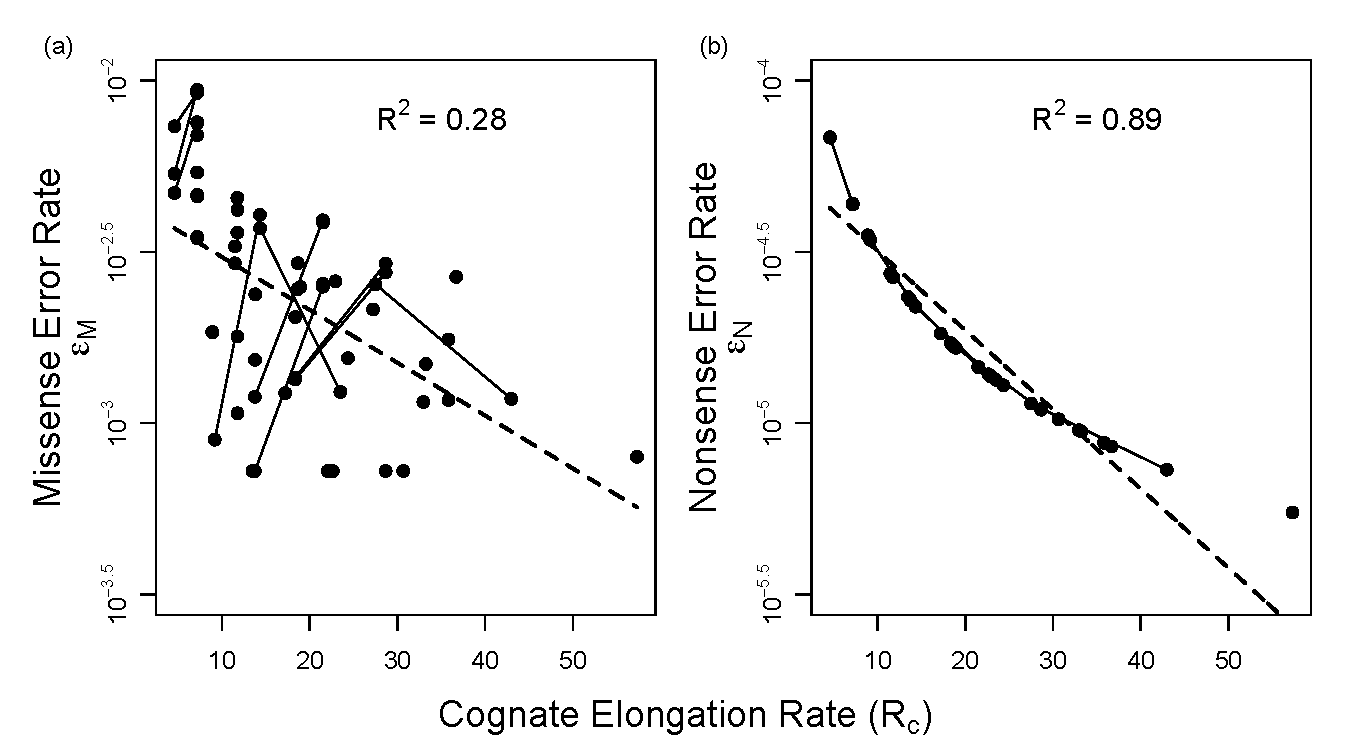
\includegraphics[width=0.49\textwidth]{../Figure/low_b_ecoli_miss_nons_vs_rc.pdf}}
                \subfloat[$R_{d}=3.146\times10^{-2}$]{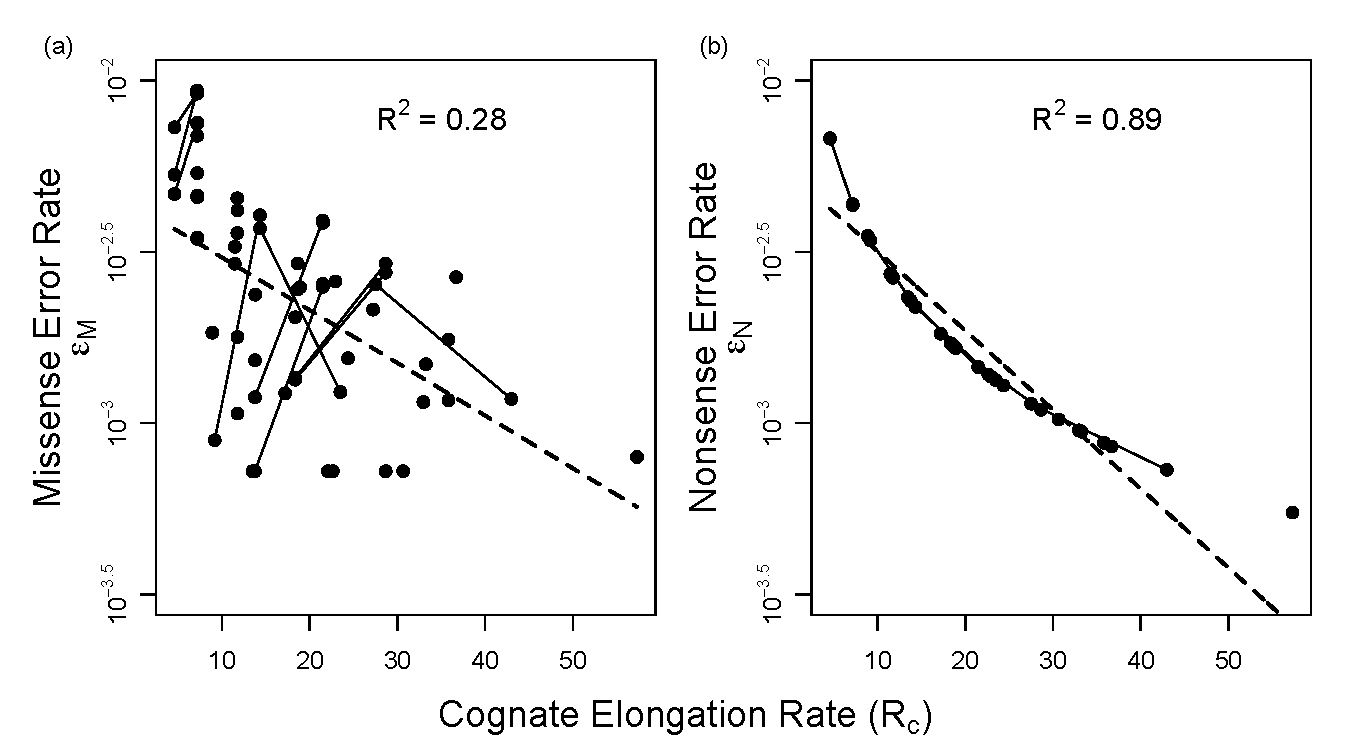
\includegraphics[width=0.49\textwidth]{../Figure/high_b_ecoli_miss_nons_vs_rc.pdf}}\vspace{2cm} 
%\end{figure}
%\begin{figure}[H]
%        \centering
                \subfloat[$w_{RR}=0.8,w_{RY}=0.64$]{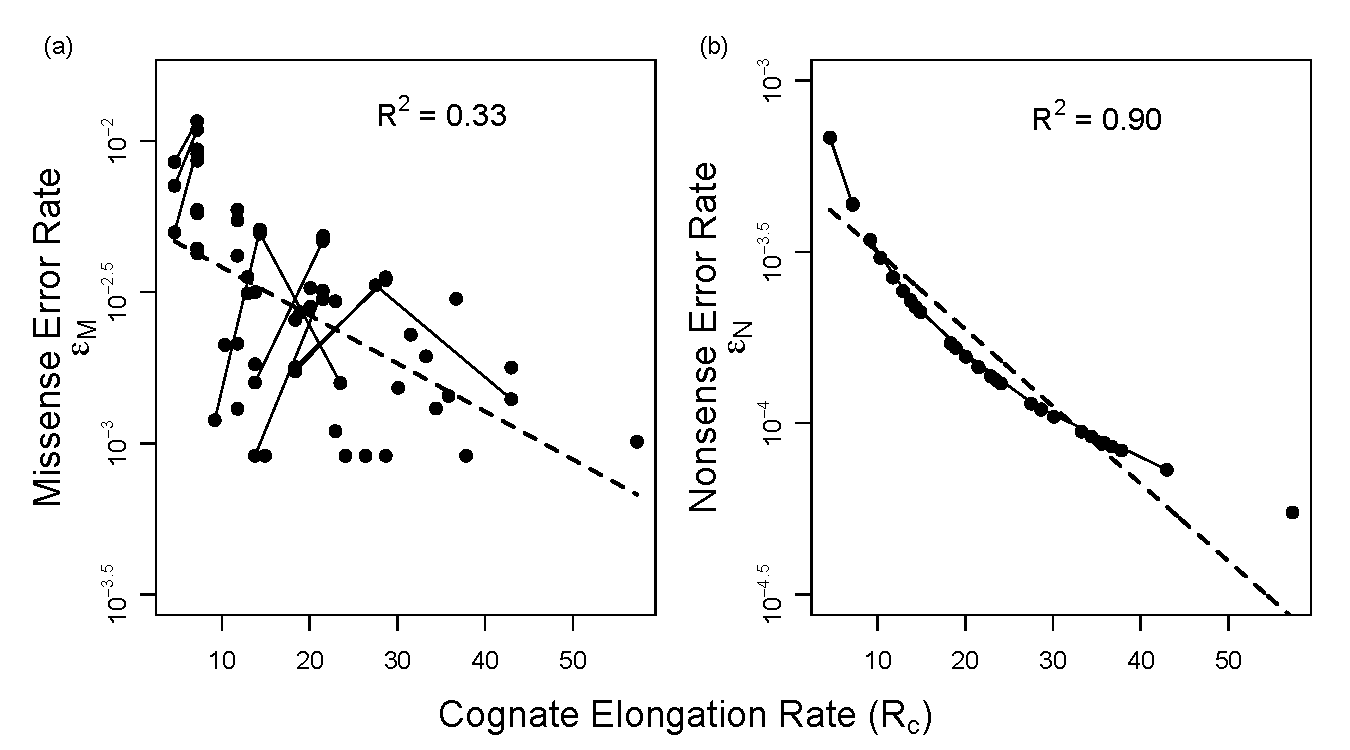
\includegraphics[width=0.49\textwidth]{../Figure/rr_0_8_ecoli_miss_nons_vs_rc.pdf}} 
                \subfloat[$w_{RR}=0.4,w_{RY}=0.64$]{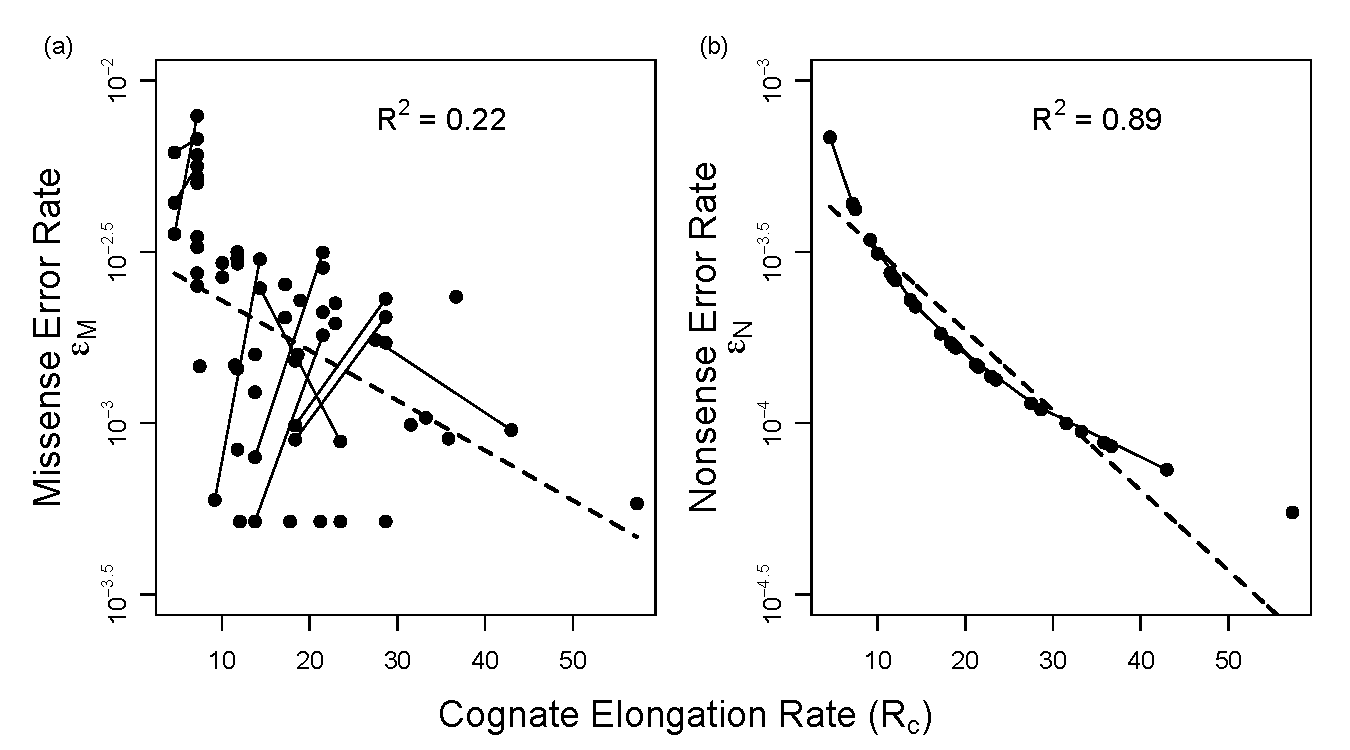
\includegraphics[width=0.49\textwidth]{../Figure/rr_0_4_ecoli_miss_nons_vs_rc.pdf}}\vspace{2cm} 
                \subfloat[$w_{RR}=0.6,w_{RY}=0.8$]{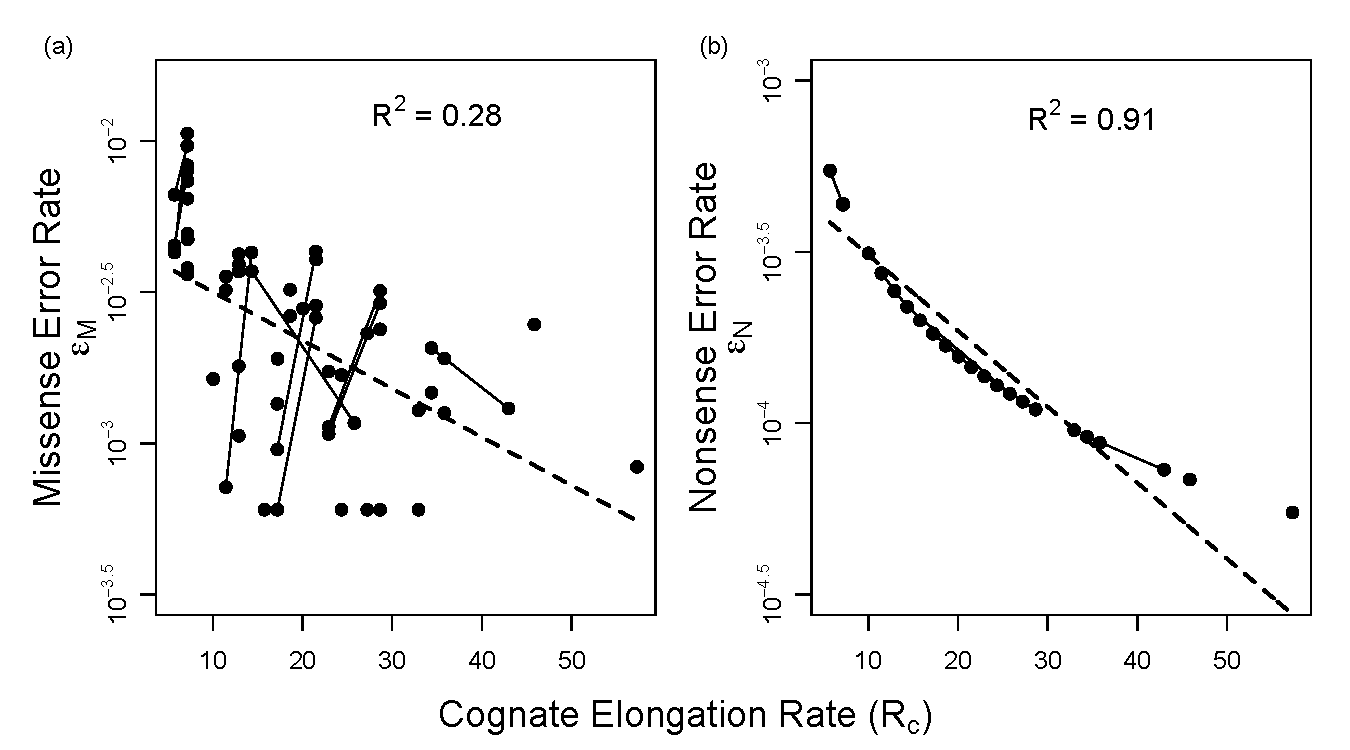
\includegraphics[width=0.49\textwidth]{../Figure/ry_0_8_ecoli_miss_nons_vs_rc.pdf}} 
                \subfloat[$w_{RR}=0.6,w_{RY}=0.4$]{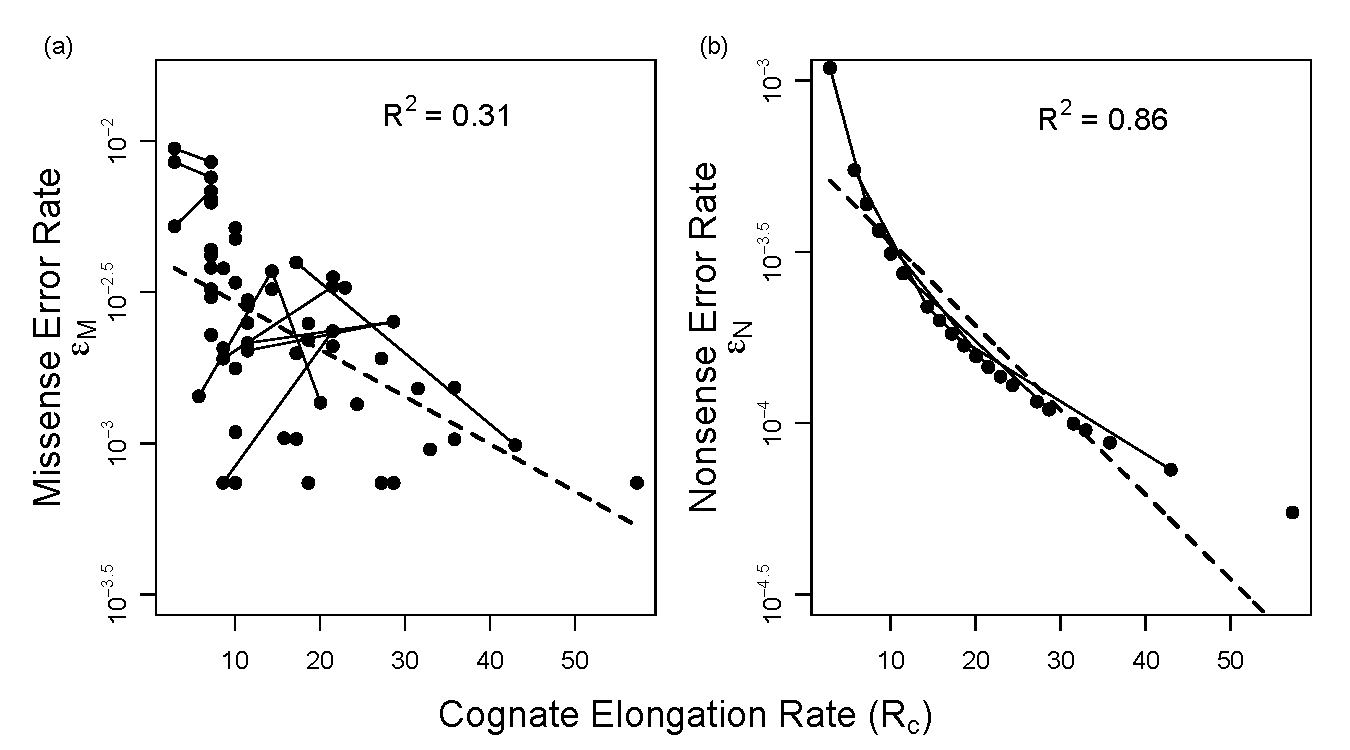
\includegraphics[width=0.49\textwidth]{../Figure/ry_0_4_ecoli_miss_nons_vs_rc.pdf}}
                \caption{Sensitivity of model behavior to changes in parameters.}
\end{figure}

\clearpage
\pagebreak

\subsection{Estimating probability of elongation at a codon during one tRNA insertion attempt} \label{sec:prob.est}

\begin{figure}[!ht]
\centering
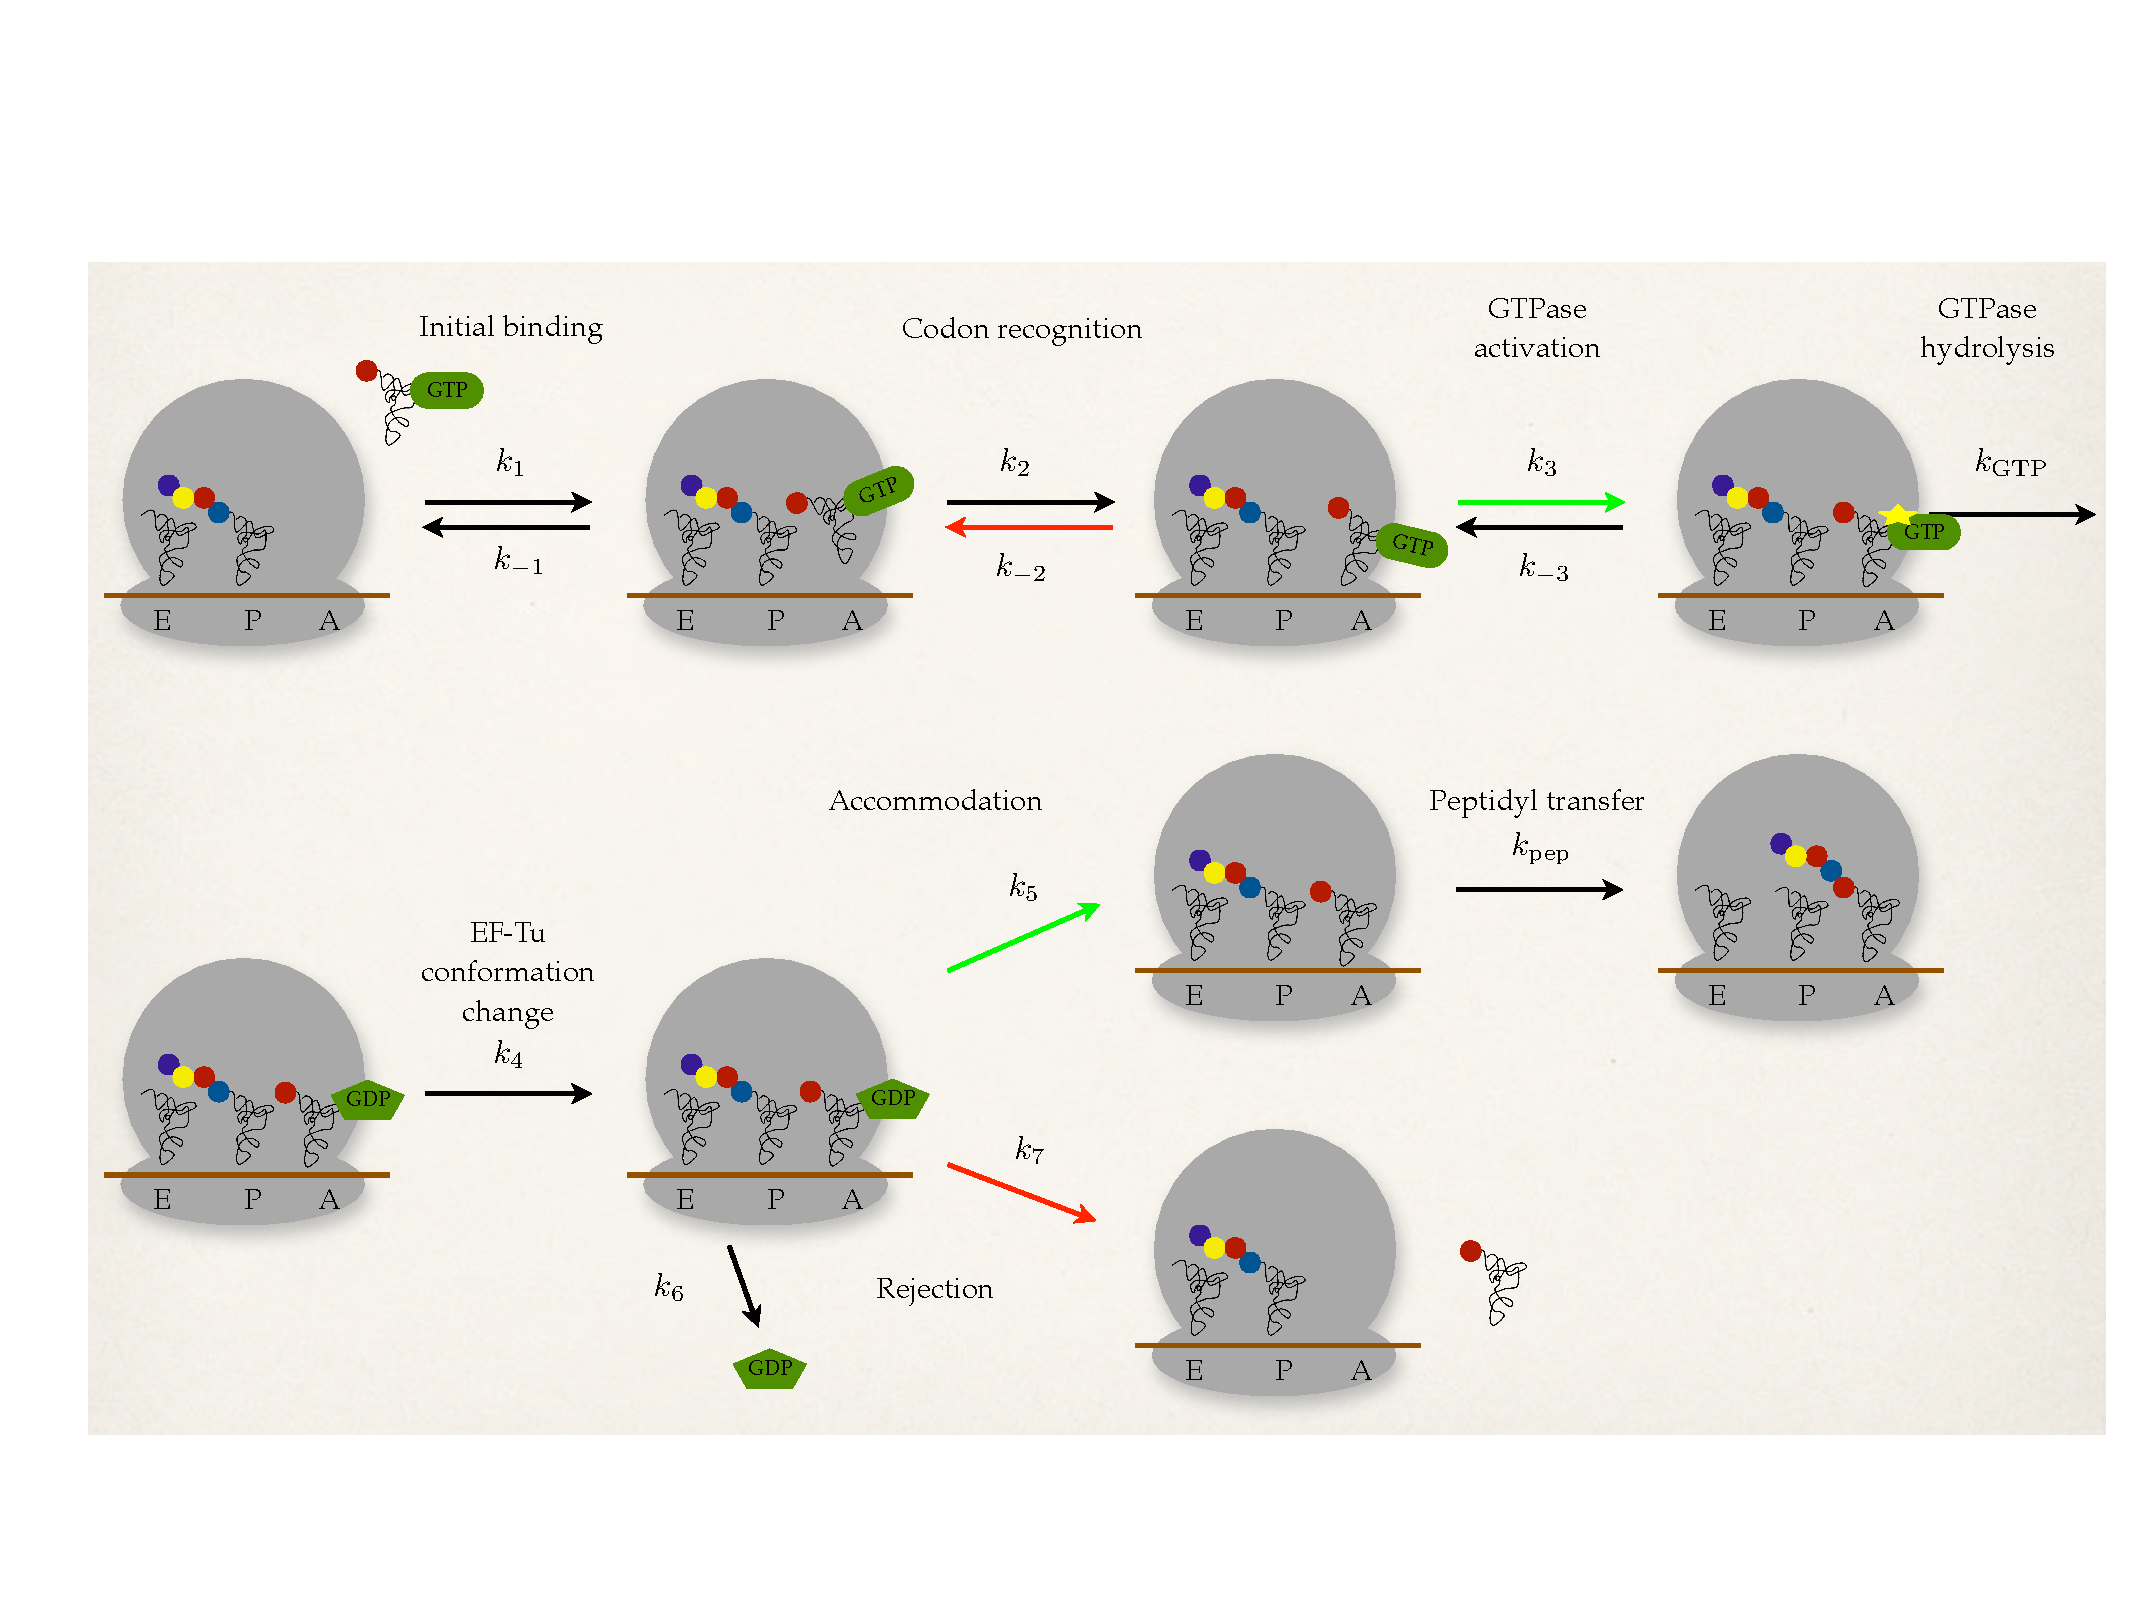
\includegraphics[width=\fullwidth]{../Figure/c2App_A1_1.pdf}
\caption{Kinetic model of tRNA selection}
The kinetic model as adapted from Gromadski and Rodnina (2004)
\end{figure}
\begin{table}[ht]
\centering
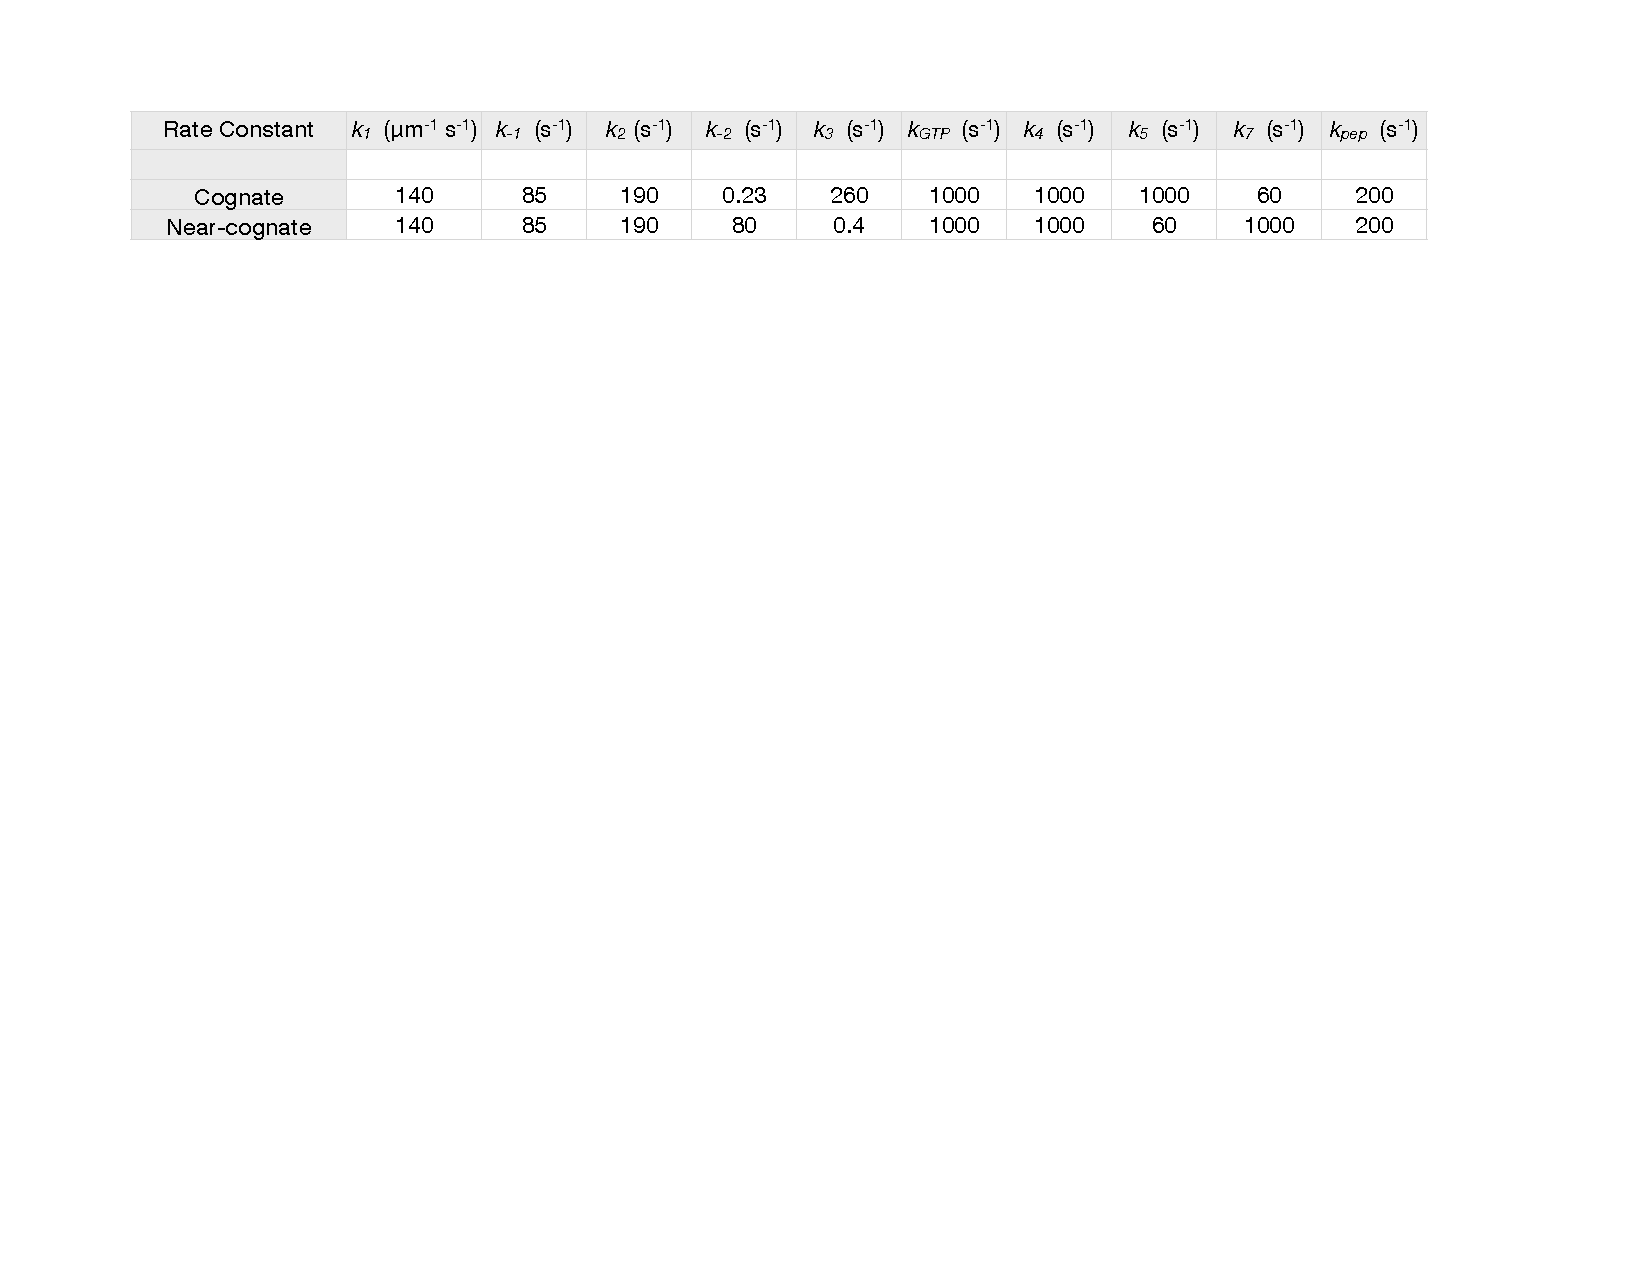
\includegraphics[width=\fullwidth]{../Figure/c2App_A1_2.pdf}
\caption{Rate constants for the kinetic model of tRNA selection}
\end{table}
%        \caption{
%         Correlation of NAI values of observed alleles versus A.) NAI values of sequences simulated under the observed protein production rate, B.) NAI values of sequences simulated under the noisy estimates of observed protein production rate and C.) NAI values of sequences simulated under the protein production rate estimated using SEMPPR \citepp{Gilchrist07}.
%         }        
Using Eqn. (5) from Fluitt, et.al. (2007), we estimated the probability of elongation as
\begin{align}
p&=\frac{P_{23}P_{34}P_{67}}{P_{23}P_{34}+P_{21}}
\end{align}
 \begin{align} 
\begin{split} 
P_{23}=\frac{k_2}{k_2+k_{-1}} 
\end{split} 
\begin{split} 
P_{34}=\frac{k_3}{k_3+k_{-2}} 
\end{split}
\begin{split}
\end{split}
\begin{split}
P_{67}=\frac{k_5}{k_5+k_7}
\end{split}
\begin{split}
\end{split}
\begin{split}
P_{21}=\frac{k_{-1}}{k_{-1}+k_2}
\end{split}
\end{align} 
Plugging in the values for cognate and near-cognate tRNAs, we find  $p_c=6.52\times 10^{-1}$ and $p_{n}=6.2\times 10^{-4}$.
\pagebreak

%\pagebreak
%\section{References}
%\bibliographystyle{plos2009}
%\bibliographystyle{apalike}
%\bibliography*{./bibliography.full}




